(注意 --- 罗马数字指本注末尾的参考文献。)

长度、面积和体积这些概念，在希腊人那里本质上建立在它们对位移的不变性之上：“能重合的东西（εφαρμόξοντα）是相等的”（Eucl. El.，第一卷，“通用概念” 4）；而经典“图形”（多边形、圆锥曲线、多面体、球面等）的面积或体积的所有公式，正是通过对这一原理的巧妙运用而得到的，有时用有限分解的方法，有时用“穷竭法” (*)。用现代的语言可以说，希腊几何学家所做的事情，就是证明“集函数”——可加且在位移下不变——的存在性，只是它们仅对非常特殊类型的集合有定义。积分演算可视为对扩大这类集函数定义域这一需要的回应，而且从 Cavalieri 到 H. Lebesgue，正是这一关切一直处于分析学家研究工作的最前沿；至于位移之下的不变性，它则退居次要地位，因为该性质已成为二重或三重积分中变量替换的一般公式以及正交变换行列式等于 ±1 这一事实的平凡推论。即使在非欧几何中（尽管那里的位移群不同），观点仍然相同：一般地，Riemann 定义了面积或体积的无穷小元素（或维数 \(\geqslant3\) 时它们的类似物），即从一个 \(ds^{2}\) 出发按经典的欧氏公式得到它们，因此它们在使 \(ds^{2}\) 不变的变换下的不变性几乎是同义反复。

直到 1890 年前后，随着积分不变量理论（尤其是 H. Poincaré 与 E. Cartan 的工作）的发展，才出现了群不变测度概念的其他一些不那么直接的推广；H. Poincaré 只考虑了在空间一部分上作用的单参数群，而 E. Cartan 首先关心的是位移群，但作用在与定义它们的那个空间不同的空间中。例如，他由此（除其他结果外）确定了 (II) \(\mathbf{R}^2\) 或 \(\mathbf{R}^3\) 的直线空间上的（在位移群下不变的）不变测度 (*)；此外他还注意到，一般地说，李群上的积分不变量无非是一些特殊的微分不变量，因此可以用 Lie 的方法把它们全部确定出来。然而，在 A. Hurwitz 1897 年的基础性工作 (V) 之前，似乎没有人想到去考虑或使用群本身上的不变测度。为了构造（\(\mathbf{R}^n\) 上）在正交群下不变的多项式，Hurwitz 从这样的评注出发：对线性变换的有限群，只要取变换 \(s \cdot P\) 的平均——其中 \(P\) 是任一多项式，\(s\) 是群的元素——问题便立即解决---这使他想到，对正交群，可用关于一个不变测度的积分来代替平均；他借助 Euler 角给出的参数表示明显地写出了这个测度的表达式，但随即（与 E. Cartan 相互独立地）注意到，Lie 的方法可对每个李群给出不变测度的存在性。也许由于 20 世纪初不变量理论的衰落，Hurwitz 的思想几乎没有得到直接的回响，直到 1924 年以后，随着 I. Schur 与 H. Weyl 把 Frobenius 关于有限群线性表示的经典理论推广到紧群，这些思想才得到发掘。前者限于正交群的情形，并指出 Hurwitz 的方法如何能把特征标的经典正交关系加以推广---H. Weyl 把这一想法与 E. Cartan 关于半单李代数的工作相结合，得到了紧李群不可约表示特征标的明显表达式以及完全可约性定理 (XI \(a\))，然后，通过对“正则表示”概念作一次大胆的推广，得到了著名的 Peter-Weyl 定理，它是有限群理论中正则表示分解为其不可约分量的完美类似 (XI, b))。

早一年，O. Schreier 建立了拓扑群的一般理论，从那时起人们已经清楚，Peter--Weyl 文章中的论证对于任何可在其上定义“不变测度”的拓扑群都原封不动地保持有效。实际上，当时拓扑学与测度论的一般概念仍处于迅速发展之中，哪些拓扑群上可以指望定义不变测度、这种“测度”应当对哪些集合来定义，似乎都尚未明确划定。唯一明显的一点是，不能指望把证明李群上不变测度存在性的无穷小方法推广到一般情形。而另一个思想潮流，从关于 Lebesgue 测度的工作出发，恰好导出了更直接的进攻方法。Hausdorff 在 1914 年证明，不存在定义在 \(R^{3}\) 的所有子集上、在位移下不变且不恒为零的可加集函数，于是自然要问这一结论对 R 与 \(R^{2}\) 是否同样成立：S. Banach 在 1923 年以一种出人意料的方式解决了这个问题，他证明恰恰相反，这样的“测度”确实存在 (I)；他的方法极为巧妙，已经建立在超限归纳构造以及函数被群的元素平移后所得的“平均” \(\frac{1}{n}\sum_{k=1}^{n}f(x+\alpha_{k})\) 的考虑之上 (*)。正是类似的思想使 A. Haar 在 1933 年 (IV) 迈出了决定性的一步，证明了对于开集具有可数基的局部紧群，不变测度的存在性：他受到经典积分演算中用任意小的全等立方体的并置逼近一个体积的方法的引导，借助对角线方法，把不变测度作为一列“近似测度”的极限而得到，这一做法本质上就是我们在 Ch. VII, §1 中所用者。这一发现影响极大，特别是因为它立即使 J. von Neumann 能够就紧群解决 Hilbert 关于用纯拓扑性质（排除任何预先给定的微分结构）刻画李群的著名的“第 5 问题”。然而人们随即察觉，要有效地使用不变测度，不仅需要知道它的存在性，还需要知道它在相差一个常数因子的意义下是唯一的；这一点先由 J. von Neumann 就紧群证明，用的是通过连续函数的（类似于 Banach 的）“平均”定义 Haar 测度的方法 (VII a))；随后 J. von Neumann (VII b)) 与 A. Weil (X) 用不同的方法同时得到了局部紧群情形的唯一性，A. Weil 同时还指明了如何把 Haar 的方法推广到一般的局部紧群。也是 A. Weil（同上）得到了齐性空间上相对不变测度存在的条件，并最终证明，Hausdorff 拓扑群上（具有合理性质的）“测度”的存在性本身就蕴涵该群是局部准紧的。这些工作实质上完成了 Haar 测度的一般理论；此后唯一值得提及的新增内容是拟不变测度的概念，它大约直到 1950 年，随着局部紧群在 Hilbert 空间中的表示理论，才被明确出来。

卷积积的历史更为复杂。早在 19 世纪初人们就注意到，例如，若 \(\mathbf{F}(x,t)\) 是关于 x 与 t 的线性常系数偏微分方程的一个解，则

\[
\int_ {- \infty} ^ {+ \infty} \mathrm{F} (x - s, t) f (s) d s
\]

也是同一方程的解；事实上，早在 1820 年之前，Poisson 等人就已经利用这一想法把热方程的解写成

\[
\int_ {- \infty} ^ {+ \infty} \exp \left(- \frac {(x - s) ^ {2}}{4 t}\right) f (s) d s.\tag{1}
\]

稍后，表达式

\[
\frac {1}{2 \pi} \int_ {- \pi} ^ {+ \pi} \frac {\sin \frac {2 n + 1}{2} (x - t)}{\sin \frac {x - t}{2}} f (t) d t\tag{2}
\]

（它给出 Fourier 级数的部分和）以及 Dirichlet 对该积分当 \(n\) 趋于 \(+\infty\) 时极限的研究，提供了“正则化” \(f \mapsto \rho_n * f\) 在环面 \(\mathbf{T}\) 上的第一个例子（实际上是用一列非正的“核”，这使研究大为复杂化）；这些类似的积分表达式以“奇异积分”之名，从 P. du Bois-Reymond 到 H. Lebesgue，一直是 19 世纪末与 20 世纪初分析学家们偏爱的课题。在 \(\mathbf{R}\) 上，Weierstrass 在其多项式逼近定理的证明中使用了积分 (1)，并在此背景下给出了用正“核”序列 \(\rho_n\) （形如 \(x \mapsto c_n \rho(x/n)\)）作正则化的一般原理。在 \(\mathbf{T}\) 上，用正核作正则化的最著名的例子稍后由 Fejér 给出，从这时起，这一标准程序便成为大多数函数项级数“求和法”的基础。

然而，这些工作由于“核”与被正则化的函数二者所起作用的不对称，几乎没有揭示卷积积的代数性质。我们尤其要感谢 Volterra 强调了这一点。他对二元函数的“复合” \(\mathbf{F}*\mathbf{G}\) 作了一般研究

\[
(\mathbf {F} * \mathbf {G}) (x, y) = \int_ {x} ^ {y} \mathbf {F} (x, t) \mathbf {G} (t, y) d t,
\]

他把它视为两个矩阵之积“由有限到无限的过渡”意义上的推广 (IX)。他很早便单独挑出了 F 与 G 只依赖于 y - x 的情形（由于它在遗传性理论中的解释而称为“闭循环”的情形）；此时 H = F * G 亦然，并且若令 \(\mathrm{F}(x,y)=f(y-x)\) ，\(\mathrm{G}(x,y)=g(y-x)\) ，则

\[
\mathrm{H} (x, y) = h (y - x),
\]

其中

\[
h (t) = \int_ {0} ^ {t} f (t - s) g (s) d s,
\]

于是，当 \(t \geqslant 0\) 时，h 与函数 \(f_{1}, g_{1}\) 的卷积相合，这两个函数当 \(t \geqslant 0\) 时分别等于 f 与 g，而当 t \textless{} 0 时等于 0。

尽管如此，Volterra 所发展的代数形式体系并未揭示出与 \(\mathbf{R}\) 的群结构以及 Fourier 变换的联系。这里不是叙述后者历史的地方；但应当指出，从 Cauchy 起，处理 Fourier 积分的分析学家们主要致力于为各种“反演”公式的有效性寻找越来越弱的条件，而在一定程度上忽视了其代数性质。对 Fourier 本人的工作（以及 Laplace 关于类似积分 \(\int_0^{+\infty}e^{-st}f(t)dt\) 的工作）当然不能这样说；但这些变换本质上是在与线性问题相关的背景下引入的，因此很长时间里无人想到考虑两个 Fourier 变换的乘积也就不足为怪了（三角级数或幂级数的乘积除外，但与离散测度的卷积之间的联系在 19 世纪显然还不可能被察觉）。这一乘积以及 \(\mathbf{R}\) 上卷积的最早提及，大概见于 Tchebychef 的一篇著作 (VIII)，与概率论中的问题有关。事实上，在这门理论中，R 上两个“概率律”（总质量为 1 的正测度）的卷积 \(\mu *\nu\) 无非就是 \(\mu\) 与 \(\nu\) 的“复合”概率律（对相应“随机变量”的加法而言）。诚然，对 Tchebychef 来说，涉及的还只是具有（关于 Lebesgue 测度的）密度的概率律的卷积，因而是函数的卷积；况且它在他的工作中只是附带地出现，在 1920--1930 年之前出现它的那几部罕见著作中情况也是如此。1920 年，P. J. Daniell 在一篇当时很少受人注意的短文 (III) 中定义了 R 上两个任意测度的卷积以及这种测度的 Fourier 变换，并明确指出 Fourier 变换把卷积变成通常的乘积---这一形式体系从 1925 年起被概率学家们密集地使用，尤其是在 P. Lévy 之后。但卷积在群论中的根本重要性直到 1927 年才被 H. Weyl 完全认识到；他注意到，对紧群而言，函数的卷积扮演着有限群代数中乘法的角色，这使他随后得以定义“正则表示”；同时，他在正则化中找到了有限群代数单位元的等价物。剩下的是把所有这些观点加以综合，这由 A. Weil 的书 (X) 完成，它为其后分别构成 I. Gelfand 的赋范代数理论与广义函数卷积的那些推广铺平了道路。

Haar 测度与卷积迅速成为代数化倾向中必不可少的工具，而这一倾向如此强烈地标志着现代分析的特征；我们将在后续各卷中有机会给出它们的众多应用。我们在这些章中处理过的唯一一个应用，涉及局部紧群的闭子群（特别是离散子群）的“变动”。这一理论从 K. Mahler 在数的几何中的一个结果出发，由 C. Chabauty 于 1950 年开创，并且刚刚被 Macbeath 与 Swierczkowski (VII) 大大地发展与深化，我们在此复述了他们的主要结果。

\specsection{参考文献}

\begin{enumerate}
\def\labelenumi{(\Roman{enumi})}
\item
  S. BANACH, Sur le problème de la mesure, Fund. Math., 4 (1923), pp.~7--33.
\item
  E. CARTAN, Le principe de dualité et certaines intégrales multiples de l'espace tangentiel et de l'espace réglé, Bull. Soc. Math. France, 24 (1896), pp.~140--177 (= Œuvres complètes, v. II \(_{1}\) , pp.~265--302).
\item
  P. J. DANIELL, Stieltjes--Volterra products, Congr. Intern. des Math., Strasbourg, 1920, pp.~130--136.
\item
  A. HAAR, Der Massbegriff in der Theorie der kontinuierlichen Gruppen, Ann. of Math., (2), 34 (1933), pp.~147--169 (= Gesammelte Arbeiten, pp.~600--622).
\item
  A. HURWITZ, Ueber die Erzeugung der Invarianten durch Integration, Gött. Nachr., 1897, pp.~71--90 (= Math. Werke, v. II, pp.~546--564).
\item
  A. M. MACBEATH, S. SWIERCZKOWSKI, Limits of lattices in a compactly generated group, Canad. J. Math., 12 (1960), pp.~427--437.
\item
  J. von NEUMANN, a) Zum Haarschen Mass in topologischen Gruppen, Comp. Math., 1 (1934), pp.~106--114 (= Collected Works, v. II, n° 22); b) The uniqueness of Haar's measure, Mat. Sbornik, 1 (43) (1936), pp.~721--734 (= Collected Works, v. IV, n° 6).
\item
  P. TCHEBYCHEF, Sur deux théorèmes relatifs aux probabilités, Acta. Math., 14 (1890), pp.~305--315) (= Œuvres, v. II, pp.~481--491).
\item
  V. VOLTERRA, Leçons sur les fonctions de lignes, Paris (Gauthier-Villars), 1913.
\item
  A. WEIL, L'intégration dans les groupes topologiques et ses applications, Actual. Scient. et Ind., n° 869, Paris, Hermann, 1940 (2 \(^{e}\) éd., ibid., n° 869-1145, Paris, Hermann, 1953).
\item
  H. WEYL, a) Theorie des Darstellung kontinuierlicher halbeinfacher Gruppen durch lineare Transformationen, Math. Zeit., 23 (1925), pp.~271--309, 24 (1926), pp.~328--395 and 789--791 (= Selecta, Basel-Stuttgart (Birkhäuser), 1956, pp.~262--366); b) (with F. PETER) Die Vollständigkeit der primitiven Darstellungen einer geschlossenen kontinuierlichen Gruppe, Math. Ann., 97 (1927), pp.~737--755 (= Selecta, pp.~387--404).
\end{enumerate}

\chapter{Hausdorff 拓扑空间上的测度}

若 T 是一个集合，A 是 T 的一个子集，则只要不致引起混淆，我们就用 \(\varphi_{A}\) 表示 A 的特征函数。集合 \(\overline{R}_{+}^{T}\) ——T 上定义的（有限或非有限的）数值函数 \(\geqslant0\) 全体——将记作 \(\mathcal{F}_{+}(T)\) ，当关于 T 没有歧义时也简记为 \(F_{+}\) ；该集合总赋有其自然的序结构。回忆 \(F_{+}\) 中两个元素的乘积总有定义，这要归功于约定 \(0\cdot(+\infty)=0\) 。若 A 是 T 的子集，f 是定义在 T 上的函数，则只要不引起混淆，f 在 A 上的限制 \(f|_{A}\) 在本章中可记作 \(f_{A}\) ；对诱导测度将采用类似的记号。另一方面，若 \(f\in\mathcal{F}_{+}(A)\) ，我们将用 \(f^{0}\) 表示 f 到 T 的 0 延拓，即在 A 上与 f 相合、在 T-A 上与 0 相合的 T 上的函数。

本章所考虑的拓扑空间，除明确说明相反情形外，都假定是 Hausdorff 的。从 §1 的 No.~4 起，除 §5 外，所有测度除明确说明相反情形外都假定为正测度。

\section{拓扑空间上的前测度与测度}

\subsection{负担}

定义 1. --- 设 T 是一个集合。称从 \(\mathcal{F}_{+}(\mathrm{T})\) 到 \(\overline{\mathbf{R}}_{+}\) 中且具有下列性质的映射 p 为 T 上的负担：

\begin{enumerate}
\def\labelenumi{\alph{enumi})}
\item
  若 \(f\) 与 \(g\) 是 \(\mathcal{F}_+\) 中使 \(f \leqslant g\) 的两个元素，则 \(p(f) \leqslant p(g)\) 。
\item
  若 \(f\) 是 \(\mathcal{F}_+\) 的一个元素，而 \(t\) 是一个 \(\geqslant 0\) 的数，则 \(p(tf) = tp(f)\) 。
\item
  若 \(f\) 与 \(g\) 是 \(\mathcal{F}_+\) 的两个元素，则 \(p(f + g) \leqslant p(f) + p(g)\) 。
\item
  若 \((f_n)\) 是 \(\mathcal{F}_+\) 中元素的一个递增序列，且 \(f = \lim_{n \to \infty} f_n\) ，则 \(p(f) = \lim_{n \to \infty} p(f_n)\) 。
\end{enumerate}

若 A 是 T 的子集，我们将用 \(p(A)\) 代替 \(p(\varphi_A)\) 。

条件 \(b)\) 蕴含 \(p(0) = 0\) 。另一方面，设 \((f_n)\) 是 \(\mathcal{F}_+\) 中元素的一个序列；条件 \(c)\) 与 \(d)\) 蕴含不等式

\[
p \left(\sum_ {n} f _ {n}\right) \leqslant \sum_ {n} p (f _ {n})
\]

（可数凸性不等式）。

例如，设 T 是一个局部紧空间，\(\mu\) 是 T 上的一个正测度；则 \(\mu^{*}\) 与 \(\mu^{\bullet}\) 都是 T 上的负担。对 \(\mu^{*}\) 这由 Ch. IV, §1, No.~3 的 Props. 10, 11, 12 与 Th. 3 得出，对 \(\mu^{\bullet}\) 这由 Ch. V, §1, No.~1 的 Prop. 1 得出。

命题 1. --- 设 \((p_{\alpha})_{\alpha \in A}\) 是 T 上的一族负担。则族 \((p_{\alpha})\) （在 \(\mathcal{F}_{+}(\mathcal{F}_{+}(T))\) 中）的和与上包络都是负担。

有限族负担的和显然是负担，故只需处理上包络的情形。定义 1 的性质 \(a), b), c)\) 显然满足，剩下要证 \(d)\) 。令 \(p = \sup p_{\alpha}\) ；于是，采用定义 1 \(d)\) 的记号，

\[
p (f) = \sup _ {\alpha} p _ {\alpha} (f) = \sup _ {\alpha} \sup _ {n} p _ {\alpha} (f _ {n}) = \sup _ {n} \sup _ {\alpha} p _ {\alpha} (f _ {n}) = \sup _ {n} p (f _ {n}).
\]

定义 2. --- 设 p 是集合 T 上的一个负担。若 \(p(T) < +\infty\) ，则称 p 是有界的。若 T 是拓扑空间，则当每个 \(x \in T\) 都具有邻域 V 使 \(p(V) < +\infty\) 时，称 p 是局部有界的。

于是由 Def. 1 的性质 \(a\) 与 \(c\) 有 \(p(\mathbf{K}) < +\infty\) ，这里 \(\mathbf{K}\) 是 \(\mathbf{T}\) 的任意紧子集。特别地，若 \(\mathbf{T}\) 紧，则 \(\mathbf{T}\) 上每个局部有界的负担都是有界的。

设 \(p\) 是集合 \(T\) 上的一个负担，\(A\) 是 \(T\) 的一个子集。对每个函数 \(f \in \mathcal{F}_{+}(A)\) ，设 \(f^0\) 是 \(f\) 到 \(T\) 的 0 延拓；则映射 \(f \mapsto p(f^0)\) （定义在 \(\mathcal{F}_{+}(A)\) 上）是一个负担，称为 \(p\) 在 \(A\) 上诱导的负担，记作 \(p|_{A}\) 或 \(p_A\) 。

设 T 与 U 是两个集合，\(\pi\) 是 T 到 U 中的一个映射，p 是 T 上的一个负担。U 上的负担 \(\pi(p)\) 对 \(f \in \mathcal{F}_{+}(U)\) 的值由下式给出：

\[
\bigl (\pi (p) \bigr) (f) = p (f \circ \pi),
\]

称其为 \(p\) 在 \(\pi\) 下的像负担。

设 \(p\) 是集合 \(T\) 上的一个负担；称 \(p\) 集中于子集 \(A\) （含于 \(T\)）上，如果 \(p(T - A) = 0\) 。

引理 1. --- 若负担 \(p\) 集中于 \(\mathbf{A} \subset \mathbf{T}\) 上，则 \(p(f) = p(f\varphi_{\mathbf{A}})\) 对每个 \(f \in \mathcal{F}_{+}(\mathbf{T})\) 成立。

因为，令 \(\mathbf{T} - \mathbf{A} = \mathbf{B}\) ，则 \(p(\varphi_{\mathrm{B}}) = 0\) ；于是

\[
f \varphi_ {\mathrm{B}} \leqslant (+ \infty) \cdot \varphi_ {\mathrm{B}} = \sup _ {n \in \mathbf {N}} n \varphi_ {\mathrm{B}},
\]

故 \(p(f\varphi_{\mathrm{B}}) = 0\) ，这由 Def. 1 的性质 \(a), b), d)\) 得出。由 \(c)\) 得 \(p(f) \leqslant p(f\varphi_{\mathrm{A}}) + p(f\varphi_{\mathrm{B}}) = p(f\varphi_{\mathrm{A}})\) ，最后 \(p(f) = p(f\varphi_{\mathrm{A}})\) 由 \(a)\) 得出。

\subsection{前测度与测度}

设 T 是拓扑空间，\(\mathcal{K}\) 是 T 的紧子集按包含关系排序所成的集合。对每个 \(K\in\mathcal{K}\) ，令 \(\mathcal{M}(K;C)\) 为 K 上复测度所成的集合。对 \(\mathcal{K}\) 中使 \(K\subset L\) 的每一对 (K,L)，令 \(\iota_{KL}\) 为 \(\mathcal{M}(L;C)\) 到 \(\mathcal{M}(K;C)\) 中的映射，它使 L 上的每个测度 \(\mu\) 对应于 \(\mu_{K}\) ，即 \(\mu\) 在 K 上诱导的测度 (Ch. IV, §5, No.~7, Def. 4)。则 \(\iota_{KM}=\iota_{KL}\circ\iota_{LM}\) ，只要 K、L、M 是 T 的满足 \(K\subset L\subset M\) 的紧子集；这由诱导测度的传递性得出 (Ch. V, §7, No.~2, Prop. 4)。族 \((\mathcal{M}(K;C))_{K\in\mathcal{K}}\) 关于映射 \(\iota_{KL}\) 的逆极限的元素称为 T 上的前测度。换言之：

定义 3. --- 称拓扑空间 T 上的这样的映射 w 为前测度：它使每个紧子集 K 对应 K 上的一个测度 \(w_{K}\) ，并且具有下列性质：

若 K 与 L 是 T 的使 \(K \subset L\) 的紧子集，则测度 \((w_{\mathrm{L}})_{\mathrm{K}}\) ——即 \(w_{L}\) 在 K 上诱导的测度——等于 \(w_{K}\) 。

若所有测度 \(w_{K}\) 都是实（相应地正）的，则称前测度 w 是实（相应地正）的。

设 \(w\) 与 \(w'\) 是 \(T\) 上的两个前测度，\(t\) 是一个复数；前测度 \(w + w'\) 与 \(tw\) 由公式 \((w + w')_K = w_K + w'_K\) 、\((tw)_K = tw_K\) （\(K\) 是 \(T\) 的任意紧子集）定义。\(T\) 上的前测度显然构成一个向量空间，记作 \(\mathcal{P}(T; \mathbf{C})\) ；实前测度所成的空间记作 \(\mathcal{P}(T; \mathbf{R})\) ，或更常记作 \(\mathcal{P}(T)\) ，正前测度的凸锥记作 \(\mathcal{P}_+(T)\) 。设 \(w\) 是一个前测度；则映射 \(K \mapsto |w_K|\) 是 \(T\) 上的一个前测度 (Ch. IV, §5, No.~7, Lemma 3)，记作 \(|w|\) 。若 \(w\) 是实的，则令 \(w^{+} = \frac{1}{2} (|w| + w)\) ，\(w^{-} = \frac{1}{2} (|w| - w)\) ；这两个前测度都是正的，于是可见每个实前测度都是两个正前测度之差。显然，对 T 的每个紧子集 K 有 \((w^{+})_{\mathrm{K}} = (w_{\mathrm{K}})^{+}\) ，\((w^{-})_{\mathrm{K}} = (w_{\mathrm{K}})^{-}\) 。

向量空间 \(\mathcal{P}(\mathrm{T})\) 由锥 \(\mathcal{P}_{+}(\mathrm{T})\) 赋序。显然 \(w^{+} = \sup(w,0)\) ，\(w^{-} = \sup(-w,0)\) ；因而 \(\mathcal{P}(\mathrm{T})\) 是格序的，且 \(\sup(w,w') = w + (w' - w)^{+}\) ，\(\inf(w,w') = w - (w' - w)^{-}\) 。此外，显然

\[
\big (\sup (w, w ^ {\prime}) \big) _ {\mathbf {K}} = \sup (w _ {\mathbf {K}}, w _ {\mathbf {K}} ^ {\prime}), \quad \big (\inf (w, w ^ {\prime}) \big) _ {\mathbf {K}} = \inf (w _ {\mathbf {K}}, w _ {\mathbf {K}} ^ {\prime})
\]

对 T 的每个紧子集 K 成立。

定义 4. --- 设 w 是 T 上的一个正前测度。对每个函数 \(f \in \mathcal{F}_{+}(T)\) ，我们令

\[
w ^ {\bullet} (f) = \sup _ {K} \left(w _ {K}\right) ^ {\bullet} \left(f _ {K}\right),\tag{1}
\]

其中 K 取遍 T 的紧子集所成的集合。

对每个紧集 K，令 \(p^{K}\) 为负担 \((w_{\mathrm{K}})^{\bullet}\) 在 K 到 T 中的典范单射下的像负担；\(w^{\bullet}\) 是诸负担 \(p^{K}\) 的上包络，从而是一个负担 (No.~1, Prop. 1)。称 \(w^{\bullet}\) 为与正前测度 w 相伴的本质上积分。我们常写 \(\int^{\bullet} f dw\) 或 \(\int^{\bullet} f(t) dw(t)\) 以代替 \(w^{\bullet}(f)\) 。

注 1). --- 若 \(v\) 与 \(w\) 是两个正前测度，则 \((v + w)^{\bullet} = v^{\bullet} + w^{\bullet}\) (Ch. V, §1, No.~1, Prop. 3)。若 \(v\) 与 \(w\) 是两个复前测度，则 \(|v + w|^{\bullet} \leqslant |v|^{\bullet} + |w|^{\bullet}\) 。

命题 2. --- a) 设 w 是一个正前测度。对 T 的每个紧子集 K，负担 \((w^{\bullet})_{\mathrm{K}}\) （由 \(w^{\bullet}\) 在 K 上诱导）等于 \((w_{\mathrm{K}})^{\bullet}\) 。对每个函数 \(f \in \mathcal{F}_{+}(\mathrm{T})\) ，有关系式 \((w_{\mathrm{K}})^{\bullet}(f_{\mathrm{K}}) = w^{\bullet}(f\varphi_{\mathrm{K}})\) 及

\[
w ^ {\bullet} (f) = \sup _ {K} w ^ {\bullet} (f \varphi_ {K}).\tag{2}
\]

\begin{enumerate}
\def\labelenumi{\alph{enumi})}
\setcounter{enumi}{1}
\tightlist
\item
  反之，设 \(p\) 是 \(T\) 上满足下列条件的负担：
\end{enumerate}

\begin{enumerate}
\def\labelenumi{\arabic{enumi})}
\item
  对 T 的每个紧子集 K，存在 K 上的一个正测度 \(w_{\mathbf{K}}\) 使 \(p_{\mathbf{K}} = (w_{\mathbf{K}})^{\bullet}\) 。
\item
  对每个函数 \(f \in \mathcal{F}_{+}(\mathrm{T})\) ，\(p(f) = \sup_{\mathrm{K}} p(f\varphi_{\mathrm{K}})\) 。
\end{enumerate}

则映射 \(w: \mathbf{K} \mapsto w_{\mathbf{K}}\) 是 \(\mathbf{T}\) 上的一个正前测度，且 \(p = w^{\bullet}\) 。

我们来证 \(a\) ：设 \(g \in \mathcal{F}_{+}(K)\) ，\(g^{0}\) 是 \(g\) 到 \(T\) 的 0 延拓；则由诱导负担的定义，

\[
(w ^ {\bullet}) _ {K} (g) = w ^ {\bullet} \left(g ^ {0}\right) = \sup _ {L} \left(w _ {L}\right) ^ {\bullet} \left(g ^ {0} \mid L\right),
\]

其中 L 取遍 T 的紧子集所成的集合，或仅仅取遍其中包含 K 的那些。但若 L 包含 K，则 \((w_{\mathrm{L}})^{\bullet}(g^{0}|\mathrm{L})=(w_{\mathrm{K}})^{\bullet}(g)\) ，因为 \(g^{0}|L\) 在 K 之外为零 (Ch. V, §7, No.~1, Prop. 1)，这就证明了第一个断言。于是

\[
(w _ {K}) ^ {\bullet} (f _ {K}) = (w ^ {\bullet}) _ {K} (f _ {K}) = w ^ {\bullet} \left((f _ {K}) ^ {0}\right) = w ^ {\bullet} (f \varphi_ {K})
\]

对一切 \(f \in \mathcal{F}_{+}(\mathrm{T})\) 成立，而 (2) 不过是把公式 (1) 转述了一遍。

转到 \(b\) ：1) 中所考虑的测度 \(w_{\mathbf{K}}\) 是唯一的 (Ch. V, §1, No.~1)。我们来证映射 \(\mathbf{K} \mapsto w_{\mathbf{K}}\) 是一个前测度：设 \(\mathbf{K}\) 与 \(\mathbf{L}\) 是使 \(\mathbf{K} \subset \mathbf{L}\) 的两个紧子集，\(\lambda\) 是 \(w_{\mathbf{L}}\) 在 \(\mathbf{K}\) 上诱导的测度；一切归结为证明 \(\lambda^{\bullet} = (w_{\mathbf{K}})^{\bullet}\) 。而 \(\lambda^{\bullet} = ((w_{\mathbf{L}})^{\bullet})_{\mathbf{K}}\) (Ch. V, §7, No.~1, Prop. 1)；由于 \((w_{\mathbf{L}})^{\bullet} = p_{\mathbf{L}}\) ，故 \(\lambda^{\bullet} = (p_{\mathbf{L}})_{\mathbf{K}} = p_{\mathbf{K}} = (w_{\mathbf{K}})^{\bullet}\) 。

用 \(w\) 表示前测度 \(K \mapsto w_K\) ；由于 \(p_K = (w_K)^{\bullet} = (w^{\bullet})_K\) ，有 \(p(f\varphi_K) = p_K(f_K) = (w^{\bullet})_K(f_K) = w^{\bullet}(f\varphi_K)\) 。于是两个负担 \(p\) 与 \(w^{\bullet}\) 相等，这由公式 (2) 以及关于 \(p\) 的假设 2) 得出。

证毕。

由于诱导负担 \((w^{\bullet})_{\mathbf{K}}\) 等于 \((w_{\mathbf{K}})^{\bullet}\) ，直接写 \(w_{\mathbf{K}}^{\bullet}\) 不会产生歧义。今后我们将采用这一记号。

推论. --- 设 v 与 w 是 T 上的两个正前测度，使得对 T 的每个紧子集 L 有 \(v^{\bullet}(\mathbf{L}) = w^{\bullet}(\mathbf{L})\) ；则 v = w。特别地，关系 \(v^{\bullet} = w^{\bullet}\) 蕴含 v = w。

因为，设 K 是 T 中的一个紧集；对每个紧集 \(L \subset K\) ，有关系式

\[
w _ {\mathrm{K}} (\mathrm{L}) = w _ {\mathrm{K}} ^ {\bullet} (\mathrm{L}) = w ^ {\bullet} (\mathrm{L}) = v ^ {\bullet} (\mathrm{L}) = v _ {\mathrm{K}} ^ {\bullet} (\mathrm{L}) = v _ {\mathrm{K}} (\mathrm{L})
\]

（由 Prop. 2）；故 \(w_{\mathrm{K}} = v_{\mathrm{K}}\) (Ch. IV, §4, No.~10, Prop. 19 的 Cor. 3)，最后由前测度的定义得 \(w = v\) 。

定义 5. --- 设 w 是拓扑空间 T 上的一个前测度。若负担 \(|w|^{\bullet}\) 是局部有界（相应地有界）的 (cf.~No.~1, Def. 2)，则称 w 是一个测度（相应地有界测度）。

\(\mathbf{T}\) 上复测度所成的集合显然是一个向量空间（注 1），记作 \(\mathcal{M}(\mathbf{T};\mathbf{C})\) 。实测度所成的空间记作 \(\mathcal{M}(\mathrm{T};\mathbf{R})\) ，或更常记作 \(\mathcal{M}(\mathrm{T})\) ，正测度的锥记作 \(\mathcal{M}_{+}(\mathrm{T})\) 。

若 w 是一个复测度，则其实部与虚部都是实测度。若 w 是一个实测度，则 \(w^{+}\) 与 \(w^{-}\) 都是正测度。于是每个复（相应地实）测度都是正测度的一个线性组合（相应地差）。

注记. --- 2) 若 T 局部紧，则 T 上每个前测度 w 都是测度。因为，每个 \(x \in T\) 都具有紧邻域 K，且 \(|w|^{\bullet}(K) = \|w_{K}\| < +\infty\) ，故负担 \(|w|^{\bullet}\) 局部有界。

\begin{enumerate}
\def\labelenumi{\arabic{enumi})}
\setcounter{enumi}{2}
\tightlist
\item
  对 T 的每个 Borel 子集 A（特别地对 A = T）及 T 上的每个正测度 \(\mu\) ，数 \(\mu^{\bullet}(\mathrm{A})\) 是 A 的紧子集的测度 \(\mu^{\bullet}(\mathrm{K})\) 的上确界。事实上，对 A 的每个紧子集 K 有 \(\mu^{\bullet}(\mathrm{K}) \leqslant \mu^{\bullet}(\mathrm{A})\) ；另一方面，若 \(\mathfrak{K}\) 是 T 的紧子集所成的集合，则
\end{enumerate}

\[
\mu^{\bullet}(\mathrm{A}) = \sup_{\mathrm{K}\in \mathfrak{K}}\mu_{\mathrm{K}}^{\bullet}(\mathrm{A}\cap \mathrm{K}) = \sup_{\mathrm{K}\in \mathfrak{K}}\sup_{\substack{\mathrm{L}\in \mathfrak{K}\\ \mathrm{L}\subset \mathrm{A}\cap \mathrm{K}}}\mu_{\mathrm{K}}^{\bullet}(\mathrm{L})\leqslant \sup_{\substack{\mathrm{L}\in \mathfrak{K}\\ \mathrm{L}\subset \mathrm{A}}}\mu^{\bullet}(\mathrm{L})
\]

（由 Ch. IV, §4, No.~6 的 Th. 4 的 Cor. 1）。

\subsection{测度的例子}

例 1. --- 局部紧空间上的测度。

下面的命题表明，本章的理论包含 Ch. IV 的理论。在陈述中，“测度”一词及记号 \(\mathcal{M}(\mathrm{T};\mathbf{C})\) 都取前面各章中的意义。

命题 3. --- 设 T 是局部紧空间，\(\mu\) 是 T 上的一个测度。用 W( \(\mu\) ) 表示使 T 的每个紧子集 K 对应诱导测度 \(\mu_{K}\) 的映射。则 W( \(\mu\) ) 是 T 上的一个前测度，有 W(\textbar{} \(\mu\) \textbar) = \textbar W( \(\mu\) )\textbar，且线性映射 W: \(\mu \mapsto\) W( \(\mu\) ) 是空间 \(\mathcal{M}(T;C)\) 到 T 上前测度所成空间 \(\mathcal{P}(T;C)\) 上的一个双射。此外，若 \(\mu\) 是正的，则 \(\mu^{\bullet} = (W(\mu))^{\bullet}\) 。

显然 \(\mathrm{W}(\mu)\) 是一个前测度 (Ch. V, §7, No.~2, Prop. 4)，且映射 W 是线性的。关系 \(\mathrm{W}(\mu)=0\) 表示 \(\mu\) 在 T 的每个紧集上诱导测度 0；于是 \(\mu(f)=0\) 对 \(f\in\mathcal{K}(\mathrm{T};\mathbf{C})\) 成立，从而 \(\mu=0\) ，这证明 W 是单射。剩下证 W 是满射。由于每个前测度都是正前测度的线性组合，只需对每个正前测度 w 构造一个正测度 \(\mu\) 使 \(w=\mathrm{W}(\mu)\) 。设 \(f\in\mathcal{K}(\mathrm{T})\) 是给定的函数，L 是包含 f 的支集的一个紧集；由诱导测度的定义，数 \(w_{\mathrm{L}}(f_{\mathrm{L}})\) 与 L 的选取无关，故可令 \(\mu(f)=w_{\mathrm{L}}(f_{\mathrm{L}})\) ；于是 \(\mu\) 是 \(\mathcal{K}(\mathrm{T})\) 上的一个正线性形式，即一个正测度。我们来验证 \(w = \mathrm{W}(\mu)\) ；首先，关系式 \(\mu^{\bullet}(f) = w_{\mathrm{L}}^{\bullet}(f_{\mathrm{L}})\) 可推广到 \(f\) 是有限的正上半连续函数且在 \(\mathbf{L}\) 之外为零的情形。因为，设 \(\mathbf{M}\) 是 \(\mathbf{L}\) 的一个紧邻域，\(\mathcal{H}\) 是 \(\mathbf{T}\) 上支集含于 \(\mathbf{M}\) 且 \(\geqslant f\) 的连续函数所成的（递减定向）集合。则 (Ch. IV, §4, No.~4, Prop. 5 的 Cor. 2)

\[
\mu^ {\bullet} (f) = \inf _ {h \in \mathscr {H}} \mu (h) = \inf _ {h \in \mathscr {H}} w _ {\mathrm{M}} (h _ {\mathrm{M}}) = w _ {\mathrm{M}} ^ {\bullet} (f _ {\mathrm{M}}),
\]

另一方面，\(w_{\mathrm{M}}^{\bullet}(f_{\mathrm{M}}) = w_{\mathrm{L}}^{\bullet}(f_{\mathrm{L}})\) ，因为 \(f_{M}\) 在 M-L 上为零 (Ch. V, §7, No.~1, Prop. 1)。特别地，若把 f 取为 \(\mathcal{K}_{+}(\mathrm{L})\) 中元素经 0 延拓所得的函数，则由诱导测度的定义，此式表明 \(\mu_{L} = w_{L}\) ，从而确实有 \(\mathrm{W}(\mu) = w\) 。

若 \(\mu\) 是正的，则

\[
\mu^ {\bullet} (f) = \sup _ {K} \mu^ {\bullet} (f \varphi_ {K}) = \sup _ {K} \mu_ {K} ^ {\bullet} (f _ {K}) = (W (\mu)) ^ {\bullet} (f)
\]

对每个 \(f \in \mathcal{F}_{+}(\mathrm{T})\) 成立 (Ch. V, §1, Def. 1 与 §7, Prop. 1)。关系 \(|\mathrm{W}(\mu)| = \mathrm{W}(|\mu|)\) 是明显的 (Ch. IV, §5, No.~7, Lemma 3)。

证毕。

当 T 局部紧时，今后我们将借助双射 W 把空间 \(\mathcal{M}(\mathrm{T};\mathbf{C})\) 与 \(\mathcal{P}(\mathrm{T};\mathbf{C})\) 等同起来。

例 2. --- 拓扑空间上具有紧支集的测度。

引理 2. --- 设 T 是拓扑空间，L 是 T 的紧子集，\(\lambda\) 是 L 上的一个正测度。则存在 T 上唯一的正测度 \(\mu\) ，使得对每个函数 \(f \in \mathcal{F}_{+}(\mathrm{T})\) 有

\[
\mu^ {\bullet} (f) = \lambda^ {\bullet} (f _ {L}).\tag{2}
\]

令 \(p(f) = \lambda^{\bullet}(f_{\mathrm{L}})\) （对每个 \(f \in \mathcal{F}_{+}(\mathrm{T})\)），我们来证 Prop. 2 b) 的条件 1) 与 2) 得到满足。第二个条件显然满足：因为 \(p(f) = p(f\varphi_{\mathrm{K}})\) 只要 \(\mathrm{K}\) 包含 \(\mathrm{L}\) 。若 \(\mathrm{K} \subset \mathrm{T}\) 紧，且 \(h \in \mathcal{F}_{+}(\mathrm{K})\) ，则

\[
p _ {\mathrm{K}} (h) = p \left(h ^ {0}\right) = \lambda^ {\bullet} \left(h ^ {0} \mid \mathrm{L}\right).
\]

但 \(h^0 | \mathbf{L}\) 是 \(h_{\mathbf{K} \cap \mathbf{L}}\) 到 \(\mathbf{L}\) 上的 0 延拓：故最后的表达式等于 \((\mu_{\mathbf{K}})^{\bullet}(h)\) ，其中 \(\mu_{\mathbf{K}}\) 是 \(\lambda | \mathbf{K} \cap \mathbf{L}\) 在 \(\mathbf{K} \cap \mathbf{L}\) 到 \(\mathbf{K}\) 的单射下的像 (Ch. V, §6, No.~2, Prop. 2 与 §7, No.~1, Prop. 1)，于是 \(p_{\mathbf{K}} = (\mu_{\mathbf{K}})^{\bullet}\) 。因而 Prop. 2 b) 的条件 1) 也得到满足，\(\mu\) 的存在性随之立得。

证毕。

我们称 \(\mu\) 为由 \(\lambda\) 定义的 T 上的测度。特别地，对 T 的每一点 \(x\) 可以定义测度 \(\varepsilon_x\) ；它由 \((\varepsilon_x)^{\bullet}(f) = f(x)\) （对 \(f \in \mathcal{F}_{+}(\mathrm{T})\)）刻画。

注记. --- 1) 当 T 局部紧时，\(\mu\) 是 \(\lambda\) 在 L 到 T 的单射下的像。我们将在 §2, No.~3 的例中（在处理过像测度之后）看到，这一解释对任意空间仍然有效。

\begin{enumerate}
\def\labelenumi{\arabic{enumi})}
\setcounter{enumi}{1}
\tightlist
\item
  我们还将看到，例 2 中定义的测度是 T 上具有紧支集的正测度 (No.~6, 注 2)。
\end{enumerate}

除明确说明相反情形外，今后我们只考虑正测度。在本节余下部分，T 表示一个拓扑空间，\(\mu\) 表示 T 上的一个正测度。

以下各小节中的许多结果可以推广到正前测度。这一推广留给读者。

\subsection{局部可忽略的集与函数}

定义 6. --- 称函数 \(f \in \mathcal{F}_{+}\) （相应地 T 的子集 A）对测度 \(\mu\) 是局部可忽略的，如果 \(\mu^{\bullet}(f) = 0\) （相应地 \(\mu^{\bullet}(A) = 0\) ）。称 \(\mu\) 集中于 T 的子集 A 上，如果 T - A 局部 \(\mu\) -可忽略。

注记. --- 1) 当 T 局部紧时，如此定义的概念与通常的概念一致。

\begin{enumerate}
\def\labelenumi{\arabic{enumi})}
\setcounter{enumi}{1}
\item
  在定义过可忽略集之后，我们将看到，局部可忽略集正是在 T 的每一点处的芽都是某个可忽略集之芽的那些集合 (No.~9, Prop. 14 的 Cor. 2)。
\item
  如同 Chs. IV 与 V 中那样，“局部几乎处处”一语与“除去一个局部可忽略集外”同义。
\item
  若 \(\theta\) 是一个复测度，我们说一个函数（相应地 T 的一个子集）对 \(\theta\) 局部可忽略，如果它对正测度 \(|\theta|\) 局部可忽略。
\end{enumerate}

例. --- 设 L 是 T 的紧子集，\(\lambda\) 是 L 上的一个测度，\(\mu\) 是由 \(\lambda\) 定义的 T 上的测度 (No.~3, 例 2)。公式 (3) 立即表明：函数 \(f \in \mathcal{F}_{+}(\mathrm{T})\) 局部 \(\mu\) -可忽略当且仅当 \(f_{L}\) 是 \(\lambda\) -可忽略的。

由公式 (1) 立即得出：函数 \(f \in \mathcal{F}_{+}(\mathrm{T})\) 局部 \(\mu\) -可忽略当且仅当对 T 的每个紧子集 K，\(f_{K}\) 是 \(\mu_{K}\) -可忽略的。于是局部可忽略集的性质立即化归为紧空间中可忽略集的性质，后者已在 Ch. IV 中处理。下面是一些今后将直接引用的结果。

--- 为使函数 \(f \geqslant 0\) 局部可忽略，必须且只需 \(f(t) = 0\) 局部几乎处处成立 (Ch. IV, §2, No.~3, Th. 1)。若 f 是以 Banach 空间为值的函数，则说 f = 0 局部几乎处处成立与说 \(\mu^{\bullet}(|\mathbf{f}|) = 0\) 等价；这时我们仍称 f 是局部可忽略的。

--- 局部可忽略函数 \(\geqslant0\) 的序列的和与上包络都是局部可忽略的 (loc. cit., No.~1, Prop. 2)。

--- 若 \(f\) 与 \(g\) 是两个 \(\geqslant 0\) 的函数且局部几乎处处相等，则 \(\mu^{\bullet}(f) = \mu^{\bullet}(g)\) (loc. cit., No.~3, Prop. 6)。

\subsection{可测集与可测函数}

定义 7. --- 设 f 是定义在 T 上、以拓扑空间 F（Hausdorff 与否均可）为值的函数。则称 f 对测度 \(\mu\) 可测（或称 \(\mu\) -可测），如果对 T 的每个紧子集 K，函数 \(f_{K}\) 是 \(\mu_{K}\) -可测的。

这等于说，对每个紧集 K，存在把 K 分解为一个 \(\mu_{K}\) -可忽略集 N 与一列紧集 \((K_{n})\) 的划分，使 f 到每个 \(K_{n}\) 的限制连续。由于说 N 是 \(\mu_{K}\) -可忽略的与说它局部 \(\mu\) -可忽略是等价的 (No.~4)，可见 f 是 \(\mu\) -可测的当且仅当对每个紧集 K，存在把 K 分解为一个局部 \(\mu\) -可忽略集 N 与一列紧集 \((K_{n})\) 的划分，使对一切 n，\(f_{K_{n}}\) 连续。~这一定义与 Ch. IV, §5, No.~1 的 Def. 1 相同，因而当 T 局部紧时重新得到通常的可测函数概念。

若 T 的子集 A 的特征函数可测，则称 A 可测。当 A 是 \(\mu\) -可测的且 \(\mu^{\bullet}(A) < +\infty\) 时，这个数简记为 \(\mu(A)\) ，称为 A 的测度。类似地，\(\mu(f)\) 表示 \(\mu^{\bullet}(f)\) ，只要 f 是 \(\geqslant 0\) 、\(\mu\) -可测且 \(\mu^{\bullet}(f) < +\infty\) 的函数。

若 \(\theta\) 是 \(\mathbf{T}\) 上的一个复测度，则称函数 \(f\) （相应地 \(\mathbf{T}\) 的子集）是 \(\theta\) -可测的，如果它对正测度 \(|\theta|\) 可测。下面的结果可以推广到复测度。

例. --- 设 L 是 T 的紧子集，\(\lambda\) 是 L 上的一个测度，\(\mu\) 是由 \(\lambda\) 定义的 T 上的测度 (No.~3, 例 2)。定义在 T 上的函数 f 是 \(\mu\) -可测的当且仅当 \(f_{L}\) 是 \(\lambda\) -可测的。因为，这一条件显然必要。反之，若它满足，则存在把 L 分解为一个 \(\lambda\) -可忽略集 N 与一列紧集 \((L_{n})\) 的划分，使对一切 n，\(f_{L_{n}}\) 连续。~若 K 是 T 的紧子集，则集合 \(K - \bigcup_{n}(K \cap L_{n})\)
与 L 的交是 \(\lambda\) -可忽略的，于是由 No.~3 的公式 (3)，该集是 \(\mu\) -可忽略的，且对一切 n，f 到 \(K \cap L_{n}\) 的限制连续。

Def. 7 使我们能够把关于可测函数的若干结果不加新证明地推广到空间非局部紧的情形。下面是其中一些今后将直接引用的结果：T 的开集与闭集都是 \(\mu\) -可测的；\(\mu\) -可测集构成一个部族 (Ch. IV, §5, No.~4, Th. 2 的 Cor. 2)，它包含 T 的 Borel 集 (loc. cit., Cor. 3) 以及 Souslin 集 (Ch. IV, §5, No.~1, Prop. 3 的 Cor. 2) \(^{(1)}\) 。数值函数的通常代数运算保持可测性 (Ch. IV, §5, No.~3)，可数的取极限运算亦然 (loc. cit., No.~4, Th. 2 与 Cor. 1)。下列性质值得更明确地指出：

命题 4. --- 设 \(f\) 是一个正函数，\((g_n)_{n \geqslant 1}\) 是一列 \(\mu\) -可测的正函数（定义在 \(T\) 上）。令 \(g = \sum_{n \geqslant 1} g_n\) ，则有

\[
\mu^ {\bullet} (f g) = \sum_ {n \geqslant 1} \mu^ {\bullet} (f g _ {n}).\tag{4}
\]

令 \(h_n = \sum_{i=1}^{n} g_i\) （对所有 \(n \geqslant 1\)）。对每个紧子集 \(K\) ⊂ \(T\)，

\[
\mu_ {\mathrm{K}} ^ {\bullet} \big ((f h _ {n}) _ {\mathrm{K}} \big) = \sum_ {i = 1} ^ {n} \mu_ {\mathrm{K}} ^ {\bullet} \big ((f g _ {i}) _ {\mathrm{K}} \big)
\]

（由应用于紧空间 K 的 Ch. V, §1, No.~1 的 Prop. 2）。关于 T 的紧子集的递增定向集取极限，即得

\[
\mu^ {\bullet} (f h _ {n}) = \sum_ {i = 1} ^ {n} \mu^ {\bullet} (f g _ {i}).
\]

而 \(fg\) 是递增序列 \((fh_n)_{n\geqslant 1}\) 的极限，故 \(\mu^{\bullet}(fg) = \lim_{n\to \infty}\mu^{\bullet}(fh_n)\) ；于是前面的公式立即蕴含 (4)。

推论. --- 设 \((\mathbf{A}_{n})\) 是两两不相交的可测子集序列，其并为 A。对 T 的每个子集 B，

\[
\mu^ {\bullet} (\mathrm{A} \cap \mathrm{B}) = \sum_ {n} \mu^ {\bullet} (\mathrm{A} _ {n} \cap \mathrm{B})
\]

特别地，

\[
\mu^ {\bullet} (\mathrm{A}) = \sum_ {n} \mu^ {\bullet} (\mathrm{A} _ {n}).
\]

在如上推广到 Hausdorff 空间的可测函数或可测集的性质中，我们还引用 Ch. IV, §5, No.~8 的 Prop. 12（紧集的 \(\mu\) -稠密族）。于是，以拓扑空间（Hausdorff 与否均可）为值的函数 f 是 \(\mu\) -可测的当且仅当 T 中使 \(f_{K}\) 连续的紧子集 K 所成的集合是 \(\mu\) -稠密的 (loc. cit., No.~10, Prop. 15)。

\subsection{定向族；测度的支集}

命题 5. --- a) 设 H 是由在 T 的每个紧子集上下半连续的 \(\geqslant 0\) 的函数组成的递增定向集。则

\[
\mu^ {\bullet} \left(\sup _ {h \in \mathrm{H}} h\right) = \sup _ {h \in \mathrm{H}} \mu^ {\bullet} (h).\tag{5}
\]

\begin{enumerate}
\def\labelenumi{\alph{enumi})}
\setcounter{enumi}{1}
\tightlist
\item
  设 H 是由在 T 的每个紧子集上上半连续的 \(\geqslant0\) 的函数组成的递减定向集。若 H 中存在函数 \(h_{0}\) 使 \(\mu^{\bullet}(h_{0})<+\infty\) ，则
\end{enumerate}

\[
\mu^ {\bullet} \left(\inf _ {h \in \mathrm{H}} h\right) = \inf _ {h \in \mathrm{H}} \mu^ {\bullet} (h).\tag{6}
\]

对每个紧集 \(\mathbf{K} \subset \mathbf{T}\) ，在情形 \(a\) ) 我们有

\[
\mu^ {\bullet} \Big (\sup _ {h \in \mathrm{H}} h \varphi_ {\mathrm{K}} \Big) = \mu_ {\mathrm{K}} ^ {\bullet} \Big (\sup _ {h \in \mathrm{H}} h _ {\mathrm{K}} \Big) = \sup _ {h \in \mathrm{H}} \mu_ {\mathrm{K}} ^ {\bullet} (h _ {\mathrm{K}}) = \sup _ {h \in \mathrm{H}} \mu^ {\bullet} (h \varphi_ {\mathrm{K}}),
\]

而在情形 \(b\)

\[
\mu^ {\bullet} \Big (\inf _ {h \in \mathrm{H}} h \varphi_ {\mathrm{K}} \Big) = \mu_ {\mathrm{K}} ^ {\bullet} \Big (\inf _ {h \in \mathrm{H}} h _ {\mathrm{K}} \Big) = \inf _ {h \in \mathrm{H}} \mu_ {\mathrm{K}} ^ {\bullet} (h _ {\mathrm{K}}) = \inf _ {h \in \mathrm{H}} \mu^ {\bullet} (h \varphi_ {\mathrm{K}}),
\]

（由 No.~2 的 Prop. 2 以及 Ch. V, §1, No.~2 的 Prop. 8）。情形 a) 通过关于 K 取上确界 (No.~2, Prop. 2) 立即得出。为处理情形 b)，用 \(\varepsilon\) 表示一个数 \(>0\) ，并选取紧集 K 使 \(\mu^{\bullet}(h_0\varphi_{\mathbf{K}}) \geqslant \mu^{\bullet}(h_0) - \varepsilon\) 。于是有 (No.~5, Prop. 4) \(\mu^{\bullet}(h_0\varphi_{\mathbf{C}_{\mathbf{K}}}) \leqslant \varepsilon\) ；故对每个函数 \(h \in \mathbf{H}\) ，只要它 \(\leqslant h_0\) ，就有 \(\mu^{\bullet}(h\varphi_{\mathbf{C}_{\mathbf{K}}}) \leqslant \varepsilon\) ，最后由 No.~5 的 Prop. 4 得 \(\mu^{\bullet}(h\varphi_{\mathbf{K}}) \geqslant \mu^{\bullet}(h) - \varepsilon\) 。于是

\[
\mu^ {\bullet} \left(\inf _ {h \in \mathrm{H}} h\right) \geqslant \mu^ {\bullet} \left(\inf _ {h \in \mathrm{H}} h \varphi_ {\mathrm{K}}\right) = \inf _ {h \in \mathrm{H}, h \leqslant h _ {0}} \mu^ {\bullet} (h \varphi_ {\mathrm{K}}) \geqslant \inf _ {h \in \mathrm{H}, h \leqslant h _ {0}} \mu^ {\bullet} (h) - \varepsilon .
\]

因此 (6) 的左端 \(\geqslant\) 右端；反向不等式是明显的，命题得证。

推论. --- a) 设 \((\mathrm{U}_{\alpha})_{\alpha \in \mathrm{I}}\) 是 T 的开子集的一个递增定向族，其并为 U。则 \(\mu^{\bullet}(\mathrm{U}) = \sup_{\alpha \in \mathrm{I}} \mu^{\bullet}(\mathrm{U}_{\alpha})\) 。

\begin{enumerate}
\def\labelenumi{\alph{enumi})}
\setcounter{enumi}{1}
\tightlist
\item
  设 \((\mathbf{F}_{\alpha})_{\alpha \in \mathbf{I}}\) 是 \(\mathbf{T}\) 的闭子集的一个递减定向族，其交为 \(\mathbf{F}\) 。若存在 \(\alpha \in \mathbf{I}\) 使 \(\mu^{\bullet}(\mathbf{F}_{\alpha})\) 有限，则 \(\mu^{\bullet}(\mathbf{F}) = \inf_{\alpha \in \mathbf{I}} \mu^{\bullet}(\mathbf{F}_{\alpha})\) 。
\end{enumerate}

由前面的推论，存在一个最大的局部可忽略开集；这证明了下述定义的合理性：

定义 8. --- T 上测度 \(\mu\) 的支集定义为 T 中最大的局部 \(\mu\) -可忽略开集的余集。

\(\mu\) 的支集记作 \(\operatorname{Supp}(\mu)\) 。

注记. --- 1) 若 \(\mu\) 是一个复测度，则 \(\mu\) 的支集定义为正测度 \(|\mu|\) 的支集；它仍是最大的局部 \(\mu\) -可忽略开集的余集。

\begin{enumerate}
\def\labelenumi{\arabic{enumi})}
\setcounter{enumi}{1}
\tightlist
\item
  我们来证明 No.~3 的例 2 中引入的测度是 T 上具有紧支集的测度。设 \(\mu\) 是 T 上的一个正测度，其支集是紧集 K，\(\nu\) 是由 \(\mu_{\mathbf{K}}\) 定义的测度（No.~3 的意义下）。设 \(f \in \mathcal{F}_{+}(\mathbf{T})\) ；则
\end{enumerate}

\[
\nu^ {\bullet} (f) = \mu_ {K} ^ {\bullet} (f _ {K}) \quad (\text { No.   3,   formula   (3)) }.
\]

由于负担 \(\mu^{\bullet}\) 集中于 K，我们还有

\[
\mu^ {\bullet} (f) = \mu^ {\bullet} (f \varphi_ {K}) = \mu^ {\bullet} ((f _ {K}) ^ {0}) = \mu_ {K} ^ {\bullet} (f _ {K}),
\]

故 \(\mu^{\bullet} = \nu^{\bullet}\) ，最后 \(\mu = \nu\) 。反之，若 K 是 T 中的紧集，\(\lambda\) 是 K 上的一个测度，而 \(\mu\) 是由 \(\lambda\) 定义的 T 上的测度，则 \(\mu^{\bullet}(\mathbb{C}K) = 0\) (No.~3, 公式 (3))；于是 \(\mu\) 的支集含于 K，从而是紧的。

\subsection{测度的上包络与和}

命题 6. --- 设 \((\lambda_{\alpha})_{\alpha \in A}\) 是 T 上的一个递增定向的测度族，令 \(p = \sup_{\alpha} \lambda_{\alpha}^{\bullet}\) 。为使族 \((\lambda_{\alpha})\) 在 \(\mathcal{M}(T)\) 中有上界，必须且只需负担 \(p\) 局部有界。此时族 \((\lambda_{\alpha})\) 有上确界 \(\lambda\) （在 \(\mathcal{M}(T)\) 中），且 \(\lambda^{\bullet} = p\) 。对每个紧集 K，测度 \(\lambda_{K}\) 都是诸测度 \((\lambda_{\alpha})_{K}\) 在 \(\mathcal{M}(K)\) 中的上确界。

若族 \((\lambda_{\alpha})\) 在 \(\mathcal{M}(\mathrm{T})\) 中有上界，则 p 显然局部有界。反之，设 p 局部有界，我们来证明它满足 No.~2 的 Prop. 2 b) 的条件 1) 与 2)。对于 2)，这由下列等式得出：

\[
p (f) = \sup _ {\alpha} \lambda_ {\alpha} ^ {\bullet} (f) = \sup _ {\alpha} \sup _ {K} \lambda_ {\alpha} ^ {\bullet} (f \varphi_ {K}) = \sup _ {K} \sup _ {\alpha} \lambda_ {\alpha} ^ {\bullet} (f \varphi_ {K}) = \sup _ {K} p (f \varphi_ {K}).
\]

另一方面，设 K 是一个紧集；负担 \(p_{K}\) 等于诸负担 \((\lambda_{\alpha}^{\bullet})_{K}\) 的上包络，且由于 p 局部有界，它是有界的。于是诸测度 \((\lambda_{\alpha})_{K}\) 有上确界 \(\lambda_{K}\) （在 \(\mathcal{M}(K)\) 中），且 \(\lambda_{K}^{\bullet}=p_{K}\) (Ch. V, §1, No.~4, Prop. 11)。这样 No.~2 的 Prop. 2 b) 的条件 1) 得以满足，因此存在 T 上的测度 \(\lambda\) 使 \(\lambda^{\bullet}=p\) ；显然 \(\lambda\) 是诸测度 \(\lambda_{\alpha}\) 的上确界。

定义 9. --- 设 \((\mu_i)_{i \in I}\) 是 T 上的一个测度族。设 A 是 I 的有限子集全体；对每个 \(\alpha \in A\) 令 \(\lambda_\alpha = \sum_{i \in \alpha} \mu_i\) 。若族 \((\lambda_\alpha)\) 有上确界 \(\mu\) （在 \(\mathcal{M}(T)\) 中），则称族 \((\mu_i)\) 可和，\(\mu\) 称为族 \((\mu_i)\) 的和，并记 \(\mu = \sum_{i \in I} \mu_i\) 。

这一定义推广了 Ch. V, §2, No.~1 中的定义。

命题 7. --- 为使族 \((\mu_i)_{i \in I}\) 可和且其和为 \(\mu\) ，必须且只需负担 \(p = \sum_{i \in I} \mu_i^\bullet\) 局部有界，此时 \(p = \mu^\bullet\) 。于是对 T 的每个紧子集 K，族 \(\left((\mu_i)_K\right)_{i \in I}\) 在 \(\mathcal{M}(K)\) 中可和，且 \(\mu_K = \sum_{i \in I} (\mu_i)_K\) 。

沿用 Def. 9 的记号，有 \(\lambda_{\alpha}^{\bullet} = \sum_{i\in \alpha}\mu_{i}^{\bullet}\) （对 I 的每个有限子集 \(\alpha\)）(No.~2, 注 1)。于是所述结论是 Prop. 6 的直接推论。

关系式 \(\mu_{\mathrm{K}} = \sum_{i\in \mathrm{I}}(\mu_i)_{\mathrm{K}}\) 连同 Ch. V, §2, No.~2 的 Prop. 2 给出下列结果：

命题 8. --- 设 \(\mu\) 是 T 上一可和测度族 \((\mu_i)_{i \in I}\) 的和。为使 T 到拓扑空间 F（Hausdorff 与否均可）中的映射 \(f\) 是 \(\mu\) -可测的，必须且只需 \(f\) 是 \(\mu_i\) -可测的（对每个 \(i \in I\)）。

\subsection{破碎}

定义 10. --- 称 T 对 \(\mu\) 的破碎，或 \(\mu\) -破碎，为 T 的两两不相交紧子集的任一局部可数族 \((K_{\alpha})_{\alpha \in A}\) ，如果集 \(N = T - \bigcup_{\alpha} K_{\alpha}\) 局部 \(\mu\) -可忽略。

命题 9. --- a) 存在一个破碎 \((\mathrm{K}_{\alpha})_{\alpha \in \mathrm{A}}\) ，它是 T 对 \(\mu\) 的破碎。 b) 设 \((\mathrm{K}_{\alpha})_{\alpha \in \mathrm{A}}\) 是 T 对 \(\mu\) 的一个破碎。若 \(\mu_{\alpha}\) 是由 \(\mu_{\mathrm{K}_{\alpha}}\) 定义的 T 上的测度 (No.~3, 例 2)，则族 \((\mu_{\alpha})_{\alpha \in \mathrm{A}}\) 可和，其和等于 \(\mu\) ，且对每个函数 \(f \in \mathcal{F}_{+}(\mathrm{T})\) ，

\[
\mu^ {\bullet} (f) = \sum_ {\alpha \in A} \mu_ {\alpha} ^ {\bullet} (f) = \sum_ {\alpha \in A} \mu_ {K _ {\alpha}} ^ {\bullet} (f _ {K _ {\alpha}}). ^ {(1)}\tag{7}
\]

为使 T 到拓扑空间 G（Hausdorff 与否均可）中的映射 g 是 \(\mu\) -可测的，必须且只需 \(g_{K_{\alpha}}\) 是 \(\mu_{K_{\alpha}}\) -可测的（对每个 \(\alpha \in A\)）。

A) 破碎的存在性：

本证明是 Ch. IV, §5, No.~9 的 Prop. 14 的证明稍作修改后的重复。设 \(\mathcal{K}\) 是紧子集 \(K\) ⊂ \(T\) 且 \(\operatorname{Supp}(\mu_K) = K\) 者的全体，\(\mathcal{H}\) 是子集 \(\mathcal{L}\) ⊂ \(\mathcal{K}\) （由两两不相交的集组成，按包含关系排序）的全体。首先证明每个元素 \(\mathcal{L}\) ∈ \(\mathcal{H}\) 都局部可数。设 \(x\) 是 \(T\) 的一点，\(V\) 是 \(x\) 的开邻域且 \(\mu^\bullet(V) < +\infty\) ；设 \(\mathfrak{L}_V\) 是 \(K \in \mathfrak{L}\) 中与 \(V\) 相交者的全体。若 \((K_i)_{1 \leqslant i \leqslant n}\) 是 \(\mathfrak{L}_V\) 中互异元素的一个有限序列，则由 Prop. 4 的推论，

\[
\sum_ {i = 1} ^ {n} \mu^ {\bullet} (\mathrm{K} _ {i} \cap \mathrm{V}) = \mu^ {\bullet} \left(\mathrm{V} \cap \left(\bigcup_ {i = 1} ^ {n} \mathrm{K} _ {i}\right)\right) \leqslant \mu^ {\bullet} (\mathrm{V}),
\]

因为诸 \(K_{i}\) 两两不相交。于是，

\[
\sum_ {\mathrm{K} \in \mathfrak {L} _ {\mathrm{V}}} \mu^ {\bullet} (\mathrm{K} \cap \mathrm{V}) <   + \infty .
\]

而 \(\mu^{\bullet}(\mathbf{K}\cap \mathbf{V}) = \mu_{\mathbf{K}}^{\bullet}(\mathbf{K}\cap \mathbf{V}) > 0\) 对每个 \(\mathbf{K}\in \mathfrak{L}_{\mathbf{V}}\) 成立，因为 \(\mathbf{K}\cap \mathbf{V}\) 非空且在 \(\mathbf{K}\) 中开，而 \(\mu_{\mathbf{K}}\) 的支集是整个 \(\mathbf{K}\) ；因此 \(\mathfrak{L}_{\mathbf{V}}\) 可数，从而 \(\mathfrak{L}\) 确实局部可数。显然 \(\mathcal{H}\) 是归纳的且非空（有 \(\varnothing \in \mathcal{H}\) ）。于是设 \(\mathfrak{H}\) 是 \(\mathcal{H}\) 的一个极大元素。我们将证明集 \(\mathrm{N} = \mathrm{T} - \bigcup_{\mathrm{K}\in \mathfrak{H}}\mathrm{K}\)

局部可忽略。由 Prop. 2，只需验证对每个紧集 L 有 \(\mu^{\bullet}(\mathbf{N}\cap\mathbf{L})=0\) ，或者等价地 \(\mu_{\mathrm{L}}^{\bullet}(\mathrm{N}\cap\mathrm{L})=0\) 。我们用反证法。于是设 \(\mu_{\mathrm{L}}^{\bullet}(\mathrm{N}\cap\mathrm{L})>0\) 。由于与 L 相交的 \(\mathbf{K}\in\mathfrak{H}\) 全体可数，N∩L 是 \(\mu_{\mathrm{L}}\) -可测的；因此存在含于 N∩L 的紧集 J 使 \(\mu_{\mathrm{L}}^{\bullet}(\mathrm{J})>0\) 。设 S 是非零测度 \((\mu_{\mathrm{L}})_{\mathrm{J}}=\mu_{\mathrm{J}}\) 的支集；它含于 N，测度 \(\mu_{\mathrm{S}}\) 非零，且 \(\operatorname{Supp}(\mu_{\mathrm{S}})=\mathrm{S}\) (Ch. IV, §5, No.~7, Lemma 2)。于是集 \(\mathfrak{H}\cup\{\mathrm{S}\}\) 属于 \(\mathscr{H}\) ，与 \(\mathfrak{H}\) 的极大性矛盾。这就证明了破碎的存在性。

\begin{enumerate}
\def\labelenumi{\Alph{enumi})}
\setcounter{enumi}{1}
\tightlist
\item
  (7) 的证明：
\end{enumerate}

对每个 \(\alpha \in \mathbf{A}\) ，由 No.~3 的公式 (3) 及 No.~2 的 Prop. 2 a)，有 \(\mu_{\alpha}^{\bullet}(f) = \mu_{\mathrm{K}_{\alpha}}^{\bullet}(f_{\mathrm{K}_{\alpha}}) = \mu^{\bullet}(f\varphi_{\mathrm{K}_{\alpha}})\) ；这些公式表明负担 \(\sum_{\alpha \in \mathbf{A}} \mu_{\alpha}^{\bullet}\) \(\leqslant \mu^{\bullet}\) ，从而族 \((\mu_{\alpha})_{\alpha \in \mathbf{A}}\) 可和 (No.~7, Prop. 7)。于是只需证明 \(\mu = \sum_{\alpha \in \mathbf{A}} \mu_{\alpha}\) ，即建立公式

\[
\mu_ {\mathrm{K}} ^ {\bullet} = \sum_ {\alpha \in \mathrm{A}} (\mu_ {\alpha}) _ {\mathrm{K}} ^ {\bullet}\tag{8}
\]

对 T 的每个紧子集 K 成立。现固定 K，由 \(\alpha \in A\) 中使 \(K_{\alpha}\) 与 K 相交者所成的集 A' 可数。设 \(g \in \mathcal{F}_{+}(K)\) ；则 \(g^{0} = g^{0}\varphi_{N} + \sum_{\alpha \in A} g^{0}\varphi_{K_{\alpha}}\) ，且 \(g^{0}\varphi_{K_{\alpha}} = 0\) （对 \(\alpha \in A - A'\)）；由 No.~5 的 Prop. 4 推出 \(\mu^{\bullet}(g^{0}) = \sum_{\alpha \in A} \mu^{\bullet}(g^{0}\varphi_{K_{\alpha}})\) ，由此

\[
\mu_ {\mathrm{K}} ^ {\bullet} (g) = \mu^ {\bullet} (g ^ {0}) = \sum_ {\alpha \in \mathrm{A}} \mu^ {\bullet} (g ^ {0} \varphi_ {\mathrm{K} _ {\alpha}}) = \sum_ {\alpha \in \mathrm{A}} \mu_ {\alpha} ^ {\bullet} (g ^ {0}) = \sum_ {\alpha \in \mathrm{A}} (\mu_ {\alpha}) _ {\mathrm{K}} ^ {\bullet} (g);
\]

于是 (8) 得证。

C) 可测性：

为使定义在 T 上的函数 g 是 \(\mu\) -可测的，必须且只需它是 \(\mu_{\alpha}\) -可测的（对每个 \(\alpha \in A\)）(No.~7, Prop. 8)；而这等于说 \(g_{K_{\alpha}}\) 是 \(\mu_{K_{\alpha}}\) -可测的（对所有 \(\alpha \in A\)）(No.~5, 例)。证毕。

如同 Ch. IV, §5, No.~9 的 Prop. 14，可以要求诸紧集 \(K_{\alpha}\) 属于预先给定的 T 的紧子集的一个 \(\mu\) -稠密集。我们只需要下面这个将直接证明的结果：

命题 10. --- 若 g 是以拓扑空间 G（Hausdorff 与否均可）为值的 \(\mu\) -可测映射，则存在 T 的一个 \(\mu\) -破碎 \((\mathbf{L}_{\beta})_{\beta\in\mathbf{B}}\) ，使限制 \(g_{L_{\beta}}\) （对所有 \(\beta\in B\)）连续。

取一个破碎 \((\mathrm{K}_{\alpha})_{\alpha\in\mathrm{A}}\) （T 对 \(\mu\) 的破碎）。由于映射 g 可测，对每个 \(\alpha\in A\)，存在把 \(K_{\alpha}\) 分解为一列紧集 \((\mathrm{K}_{\alpha n})\) 与一个局部可忽略集 \(N_{\alpha}\) 的划分，使 g 到每个集 \(K_{\alpha n}\) 的限制连续。于是族 \((\mathrm{K}_{\alpha n})_{(\alpha,n)\in\mathrm{A}\times\mathbf{N}}\) 就是所求的破碎。因为它是局部可数的，且集 \(N' = N \cup \left( \bigcup_{\alpha} N_{\alpha} \right)\) 局部可忽略，这是由于一个紧集至多与可数无穷多个集 \(N_{\alpha}\) 相交。

附论. --- 设 \((\mathrm{K}_{\alpha})_{\alpha\in\mathrm{A}}\) 是 T 的一个破碎，令 \(N=T-\bigcup_{\alpha}K_{\alpha}\) 。用 \(T'\) 表示在 T 上赋予诸子空间 \(K_{\alpha}\) 的拓扑之和拓扑以及 N 上任一局部紧拓扑所得到的局部紧空间（除非特别说明相反情形，N 总是赋予离散拓扑）。对每个 \(\alpha \in A\) ，设 \(i_{\alpha}\) 是 \(K_{\alpha}\) 到 \(T'\) 中的典范单射，\(\mu_{\alpha}'\) 是 \(T'\) 上 \(\mu_{K_{\alpha}}\) 在 \(i_{\alpha}\) 下的像测度。族 \((\mu_{\alpha}')\) 可和：因为若 f 是 \(T'\) 上具紧支集的连续函数，则 Supp(f) 与 \(K_{\alpha}\) 只对有限个指标 \(\alpha\) 相交。令 \(\mu' = \sum_{\alpha \in A} \mu_{\alpha}'\) 。

由于集 N 对 \(\mu'\) 局部可忽略——因为它对每个 \(\mu'_{\alpha}\) 如此 (Prop. 9)——故族 \((\mathrm{K}_{\alpha})_{\alpha \in \mathrm{A}}\) 是一个 \(\mu'\) -破碎（对 \(\mathrm{T}'\) 而言）；而 \(\mu'\) 在 \(\mathrm{K}_{\alpha}\) 上诱导的测度显然是 \(\mu_{\mathrm{K}_{\alpha}}\)，公式 (7) 应用于 \(\mu\) 与 \(\mu'\) 表明 \(\mu^{\bullet} = \mu'^{\bullet}\) 。类似地，Prop. 9 陈述的最后一条应用于 \(\mu\) 与 \(\mu'\) 表明，两个测度 \(\mu\) 与 \(\mu'\) 的可测映射是相同的。

这两条性质使我们能把关于 \(\mu\) 的积分理论的几乎全部内容化归为对局部紧空间已建立的理论。这些考虑将在 No.~10 中展开。

下面是破碎概念的另一个应用：

命题 11. --- 设 X 是 T 的一个 \(\mu\) -可测子集。存在 X 的紧子集的一个局部可数族 \((\mathrm{L}_{\alpha})_{\alpha \in \mathbf{A}}\) ，两两不相交，使 \(\mathrm{X} - \bigcup_{\alpha \in \mathbf{A}} \mathrm{L}_{\alpha}\) 局部 \(\mu\) -可忽略。此外，若 X 是一列可测集 \((\mathrm{X}_n)\) （满足 \(\mu^{\bullet}(\mathrm{X}_n) < +\infty\)）之并，则 \(\alpha \in \mathbf{A}\) 中使 \(\mu^{\bullet}(\mathrm{L}_{\alpha}) \neq 0\) 者所成的集 B 可数，且 \(\mathrm{X} - \bigcup_{\beta \in \mathbf{B}} \mathrm{L}_{\beta}\) 局部 \(\mu\) -可忽略。

设 \(f\) 是 \(X\) 的特征函数，\((K_{\alpha})_{\alpha \in A}\) 是 \(T\) 的一个破碎，使 \(f\) 到每个 \(K_{\alpha}\) 的限制连续 (Prop. 10)。于是集 \(L_{\alpha} = K_{\alpha} \cap X\) 对每个 \(\alpha \in A\) 是紧的，而 \((L_{\alpha})_{\alpha \in A}\) 即为所求的族。转到第二条断言；显然可设诸可测集 \(X_{n}\) 不相交，且只需对其中每一个证明该断言。换句话说，必要时改变记号，可设 \(\mu^{\bullet}(X) < +\infty\) 。于是集 \(B\) ——即 \(\alpha \in A\) 中使 \(\mu^{\bullet}(L_{\alpha}) > 0\) 者——可数，剩下只要证明集 \(N = \bigcup_{\alpha \in A - B} L_{\alpha}\) 局部可忽略。设 \(K\) 是一个紧集；族

\((\mathrm{L}_{\alpha})_{\alpha\in\mathrm{A}}\) 局部可数，故集 \(\mathrm{K}\cap\mathrm{N}\) 是族 \((\mathrm{K}\cap\mathrm{L}_{\alpha})_{\alpha\in\mathrm{A}-\mathrm{B}}\) 的一个可数子族之并，从而该集局部可忽略。于是 \(\mathrm{N}\) 亦然 (No.~2, Prop. 2)，命题得证。

\subsection{上积分}

定义 11. --- 对每个函数 \(f \in \mathcal{F}_{+}(T)\) ，定义 f 的上积分（关于测度 \(\mu\) ）为有限或无限的正数

\[
\mu^ {*} (f) = \inf _ {g} \mu^ {\bullet} (g),\tag{9}
\]

其中 \(g\) 取遍 \(\geqslant f\) 的下半连续函数全体。也使用记号 \(\int^{*} f(t) d\mu(t)\) 与 \(\int^{*} f d\mu\) 。当 \(T\) 局部紧时，这一定义与通常的定义一致 (Ch. V, §1, No.~1, Prop. 4)。显然 \(\mu^{\bullet}(f) \leqslant \mu^{*}(f)\) ，且当 \(f\) 下半连续时取等号。若 \(A\) 是 \(T\) 的子集，则用 \(\mu^{*}(A)\) 代替 \(\mu^{*}(\varphi_{A})\) ，这个数称为 \(A\) 的外测度。具有有限外测度的可测集称为可积集，与局部紧空间的情形一样。

函数 \(\mathbf{f}\) 若以 Banach 空间或 \(\overline{\mathbf{R}}\) 为值且满足 \(\mu^{*}(|\mathbf{f}|)=0\) ，就称为可忽略的；集 \(A\subset T\) 称为可忽略的，如果 \(\varphi_{A}\) 可忽略，即 \(\mu^{*}(A)=0\) 。几乎处处这一说法按 Ch. IV, §2, No.~3 的方式引入。

命题 12. --- 函数 \(\mu^{*}\) 是 T 上的一个负担。

No.~1 的 Def. 1 的性质 \(a\) 、\(b\) 、\(c\) 是明显的。性质 \(d\) 的证明与 Ch. IV, §1, No.~3 的 Th. 3 的证明相同，只需顾及 Props. 4 与 5 \(a\) )。

推论. --- 以 Banach 空间或 \(\overline{R}\) 为值的函数 f 可忽略，当且仅当 \(\mathbf{f}(t)=0\) 几乎处处成立。

立即化归为正函数的情形。此后的证明与 Ch. IV, §2, No.~3 的 Th. 1 的证明相同。

命题 13. --- 对 T 的每个子集 A，\(\mu^{*}(\mathbf{A})\) 是包含 A 的诸开集的外测度的下确界。

证明与 Ch. IV, §1, No.~4 的 Prop. 19 的证明相同。

定义 12. --- 设 f 是定义在 T 上、以 Banach 空间或 \(\overline{R}\) 为值的函数。若 f 在可数个可积开集之并的余集上为零，则称 f 对测度 \(\mu\) 适度，或 \(\mu\) -适度。若函数 \(\varphi_{A}\) 适度，则称 T 的子集 A 适度。若函数 1 是 \(\mu\) -适度的，则称测度 \(\mu\) 适度。

例如，由于负担 \(\mu^{\bullet}\) 局部有界，T 的每个紧子集 K 都含于一个使 \(\mu^{\bullet}(V)<+\infty\) 的开集 V；因此在紧集外为零的函数是适度的。可忽略函数是适度的。Ch. V, §1, No.~2 中 Def. 2 后面的注记可立即推广到当前情形。特别地，一列适度正函数的和是适度的。

注记. --- 1) 在 Lindelöf 空间 T 上 (TG, IX, Appendix I, Def. 1)，\(^{1}\) 特别地在 Souslin 空间上 (ibid., Prop. 1 的 Cor.)，每个测度都是适度的。因为有限测度的开集构成 T 的一个覆盖，从中可以取出 T 的一个可数覆盖。

\begin{enumerate}
\def\labelenumi{\arabic{enumi})}
\setcounter{enumi}{1}
\tightlist
\item
  然而要注意，存在一列对 \(\mu\) 具有有限测度、并以 T 为并的 Borel 集，并不一定蕴含存在一列以 T 为并、具有限测度的开集（换句话说，不蕴含 \(\mu\) 适度）。见 Exer. 8。
\end{enumerate}

命题 14. --- 设 \(f \in \mathcal{F}_{+}(\mathrm{T})\) 。若 \(f\) 是 \(\mu\) -适度的，则 \(\mu^{*}(f) = \mu^{\bullet}(f)\) ；若 \(f\) 不是 \(\mu\) -适度的，则 \(\mu^{*}(f) = +\infty\) 。

若 \(\mu^{*}(f) < +\infty\) ，则存在下半连续函数 \(g \geqslant f\) 使 \(\mu^{\bullet}(g) < +\infty\) 。对每个 \(n \in \mathbf{N}\) ，设 \(\mathbf{G}_{n}\) 是 \(t \in \mathbf{T}\) 中使 \(g(t) > 1/n\) 者的全体；集 \(\mathbf{G}_{n}\) 是开集，有 \(\mu^{\bullet}(\mathbf{G}_{n}) \leqslant n\mu^{\bullet}(g) < +\infty\) ，且 \(f\) 在诸 \(\mathbf{G}_{n}\) 之并外为零：因此函数 \(f\) 适度。

其次，证明 \(\mu^{*}\) 与 \(\mu^{\bullet}\) 在适度函数上取相同的值。由于 \(\mu^{*}\) 与 \(\mu^{\bullet}\) 都是负担，只需对如下情形建立关系 \(\mu^{*}(f)=\mu^{\bullet}(f)\)：f 是正函数，被常数 M 控制且在一个具有限测度的开集 G 外为零；我们现在就来证明这一点。

测度 \(\mu\) 是 \(\mathcal{M}(\mathrm{T})\) 中一个由具紧支集的测度组成的递增定向族 \((\mu_i)_{i\in I}\) 的上确界：这由 No.~8 的 Prop. 9 立即得出。设 \(g\) 是 \(\mathrm{T}\) 上介于 \(f\) 与下半连续函数 \(\mathrm{M}\varphi_{\mathrm{G}}\) 之间的下半连续函数。令 \(\nu_i = \mu - \mu_i\) ；则 \(\mu^{\bullet} = \mu_i^{\bullet} + \nu_i^{\bullet}\) (No.~2, 注 1)，因此

\[
\begin{array}{r l} \mu^ {\bullet} (g) - \mu^ {\bullet} (f) & = (\mu_ {i} ^ {\bullet} (g) - \mu_ {i} ^ {\bullet} (f)) + (\nu_ {i} ^ {\bullet} (g) - \nu_ {i} ^ {\bullet} (f)) \\ & \leqslant (\mu_ {i} ^ {\bullet} (g) - \mu_ {i} ^ {\bullet} (f)) + \nu_ {i} ^ {\bullet} (\mathrm{M} \varphi_ {\mathrm{G}}). \end{array}
\]

有 \(\nu_{i}^{\bullet}(\mathrm{M}\varphi_{\mathrm{G}}) = \mu^{\bullet}(\mathrm{M}\varphi_{\mathrm{G}}) - \mu_{i}^{\bullet}(\mathrm{M}\varphi_{\mathrm{G}})\) 且 \(\mu^{\bullet}(\mathrm{M}\varphi_{\mathrm{G}}) = \sup \mu_{i}^{\bullet}(\mathrm{M}\varphi_{\mathrm{G}})\) (No.~7, Prop. 6)；因此数 \(\nu_{i}^{\bullet}(\mathrm{M}\varphi_{\mathrm{G}})\) 可通过适当选取 \(i\) 而任意小。于是问题归结为证明：对任意数 \(c > 0\) 与任意指标 \(i \in I\) ，能找到下半连续函数 \(g\) ，介于 \(f\) 与 \(\mathrm{M}\varphi_{\mathrm{G}}\) 之间，使 \(\mu_{i}^{\bullet}(g) - \mu_{i}^{\bullet}(f) \leqslant c\) 。现设 \(L\) 是测度 \(\mu_{i}\) 的紧支集，\(\lambda\) 是测度 \((\mu_{i})_{L}\) ；由于 \(\mu_{i}\) 集中于 \(L\) ，有 \(\mu_{i}^{\bullet}(h) = \mu_{i}^{\bullet}(h\varphi_{L}) = \lambda^{\bullet}(h_{L})\) （对每个函数 \(h \in \mathcal{F}_{+}(T)\)）(No.~1, Lemma 1 与 No.~2, Prop. 2)；因此

\[
\mu_ {i} ^ {\bullet} (g) - \mu_ {i} ^ {\bullet} (f) = \lambda^ {\bullet} (g _ {\mathrm{L}}) - \lambda^ {\bullet} (f _ {\mathrm{L}}).
\]

但 L 是紧的；因此 \(\lambda^{\bullet} = \lambda^{*}\) ，于是存在定义在 L 上的下半连续函数 h，它 \(\geqslant f_{L}\) 且使 \(\lambda^{\bullet}(h) \leqslant \lambda^{\bullet}(f_{\mathrm{L}}) + c\) 。由于集 L 在 T 中闭，在 L 上等于 h 而在 T - L 上等于 \(+\infty\) 的函数 k 在 T 上下半连续且 \(\geqslant f\) ，并且 \(\lambda^{\bullet}(k_{\mathrm{L}}) = \lambda^{\bullet}(h) \leqslant \lambda^{\bullet}(f_{\mathrm{L}}) + c\) 。只需令 \(g = \inf(k, M\varphi_{G})\) ：g 下半连续，\(g \geqslant f\) ，且

\[
\mu_ {i} ^ {\bullet} (g) \leqslant \mu_ {i} ^ {\bullet} (k) = \lambda^ {\bullet} (k _ {\mathrm{L}}) \leqslant \lambda^ {\bullet} (f _ {\mathrm{L}}) + c = \mu_ {i} ^ {\bullet} (f) + c.
\]

推论 1. --- 一个函数可忽略，必须且只需它局部可忽略且适度。

推论 2. --- 函数 f 局部可忽略，必须且只需每个 \(x \in T\) 都有邻域 V 使 \(f\varphi_{V}\) 可忽略。

因为若这一性质满足，则对每个紧集 K，\(f\varphi_{K}\) 可忽略，因此 f 局部可忽略 (No.~2, Prop. 2)。反之，设 f 局部可忽略，x 是 T 的一点；x 有一个具有限测度的开邻域 V。于是函数 \(f\varphi_{V}\) 局部可忽略且适度，从而可忽略。

推论 3. --- 设 \(\mathbf{f}\) 是定义在 \(\mathbf{T}\) 上的适度函数。存在两两不相交的紧集序列 \((\mathbf{K}_n)\) 与可忽略集 \(\mathbf{H}\) ，使 \(\mathbf{f} = \mathbf{f}\varphi_{\mathrm{H}} + \sum_{n} \mathbf{f}\varphi_{\mathrm{K}_n}\) 。

因为设 G 是可数个可积开集之并的集，f 在 G 外为零；则 G 是两两不相交的紧集序列 \((K_{n})\) 与一个局部可忽略集 H 的并 (No.~8, Prop. 11)；而 H 适度，因此可忽略。

推论 4. --- 若 \(\mu\) 与 \(\nu\) 是 T 上两个使 \(\mu^{*} = \nu^{*}\) 的测度，则 \(\mu = \nu\) 。

因为等式 \(\mu^{*}=\nu^{*}\) 蕴含 \(\mu^{\bullet}(f)=\nu^{\bullet}(f)\) 对每个对 \(\mu\) 与 \(\nu\) 适度的正函数 f 成立，从而对每个具紧支集的正函数成立；由此得 \(\mu^{\bullet}=\nu^{\bullet}\) (No.~2, Prop. 2)，再得 \(\mu=\nu\) (No.~2, Prop. 2 的 Cor.)。

推论 5. --- 若 \(\mu\) 是 T 上的适度测度，则存在一列具紧支集的测度 \((\mu_n)_{n \in \mathbf{N}}\) 使 \(\mu = \sum_{n \in \mathbf{N}} \mu_n\) 。

根据假设，常函数 1 是 \(\mu\) -适度的。把 Cor. 3 应用于 \(f = 1\) 的情形；于是存在 T 的两两不相交的紧子集序列 \((\mathrm{K}_n)_{n \in \mathbf{N}}\) ，使 \(1 = \sum_{n \in \mathbf{N}} \varphi_{\mathrm{K}_n}\) \(\mu\) -几乎处处成立。

设 \(\mu_{n}\) 是由测度 \(\mu_{\mathrm{K}_n}\) （在 \(\mathrm{K}_n\) 上）定义的 T 上的测度 (No.~3, 例 2)。已知 (No.~6, 注 2) \(\mu_{n}\) 具紧支集，且 \(\mu_n^\bullet (f) = \mu^\bullet (f\varphi_{\mathrm{K}_n})\) （对 \(f\in \mathcal{F}_{+}(\mathrm{T})\)）。而 \(f\) 等于 \(\sum_{n\in \mathbf{N}}f\varphi_{\mathrm{K}_n}\) （\(\mu\) -几乎处处），由此

\[
\mu^ {\bullet} (f) = \sum_ {n \in \mathbf {N}} \mu^ {\bullet} (f \varphi_ {\mathrm{K} _ {n}}) = \sum_ {n \in \mathbf {N}} \mu_ {n} ^ {\bullet} (f).
\]

于是 \(\mu = \sum_{n\in \mathbf{N}}\mu_n\) (No.~7, Prop. 7)。

\subsection{积分理论}

定义 13. --- 设 \(p \in [1, +\infty[\) ；用 \(\overline{\mathcal{L}}^p(T, \mu)\) （相应地 \(\overline{\mathcal{L}}_F^p(T, \mu)\) ，若 \(F\) 是 Banach 空间）表示映射 \(f\) （从 \(T\) 到 \(\overline{R}\) ，相应地到 \(F\) ）中 \(\mu\) -可测且满足 \(\mu^\bullet(|f|^p) < +\infty\) 者的全体。用 \(\mathcal{L}^p(T, \mu)\) （相应地 \(\mathcal{L}_F^p(T, \mu)\) ）表示 \(\mu\) -适度元素（\(\overline{\mathcal{L}}^p(T, \mu)\) 中的，相应地 \(\overline{\mathcal{L}}_F^p(T, \mu)\) 中的）全体。

我们记 \(\overline{\mathbf{N}}_p(\mathbf{f}) = (\mu^\bullet (|\mathbf{f}|^p))^{1 / p}\) ，\(\mathrm{N}_p(\mathbf{f}) = (\mu^* (|\mathbf{f}|^p))^{1 / p}\) 。用 \(\overline{\mathrm{N}}_{\infty}(\mathbf{f})\) 表示数 \(k\geqslant 0\) （使 \(|\mathbf{f}|\leqslant k\) 局部 \(\mu\) -几乎处处成立）的下确界；若 \(\overline{\mathrm{N}}_{\infty}(\mathbf{f}) < + \infty\) ，则称 \(\mathbf{f}\) 本性有界。T 到 \(\overline{\mathbf{R}}\) （相应地到 F）中的可测且本性有界的映射全体记作 \(\overline{\mathcal{L}}^{\infty}(\mathrm{T},\mu)\) （相应地 \(\overline{\mathcal{L}}_{\mathrm{F}}^{\infty}(\mathrm{T},\mu)\) ）。\(\overline{\mathcal{L}}_{\mathrm{F}}^{1}(\mathrm{T},\mu)\) （相应地 \(\mathcal{L}_{\mathrm{F}}^{1}(\mathrm{T},\mu)\)）的元素称为以 F 为值的本性可积函数（相应地可积函数）。

若 \(\mu\) 是复测度，则令

\[
\overline {{{{\mathcal {L}}}}} _ {\mathrm{F}} ^ {p} (\mathrm{T}, \mu) = \overline {{{{\mathcal {L}}}}} _ {\mathrm{F}} ^ {p} (\mathrm{T}, | \mu |) \quad \text { and } \quad \mathcal {L} _ {\mathrm{F}} ^ {p} (\mathrm{T}, \mu) = \mathcal {L} _ {\mathrm{F}} ^ {p} (\mathrm{T}, | \mu |).
\]

只要不引起混淆，上述记号常缩写为 \(\overline{\mathcal{L}}_F^p (\mu)\) 、\(\overline{\mathcal{L}}_F^p\) 或 \(\mathcal{L}^p (\mu)\) 、\(\mathcal{L}^p\) 。

我们在 No.~8（附论）中看到，可以构造一个局部紧空间 \(\mathbf{T}'\) ，它与 \(\mathbf{T}\) 有同一底层集合且拓扑比 \(\mathbf{T}\) 更细，并在 \(\mathbf{T}'\) 上配备测度 \(\mu'\) ，使 \(\mu\) -可测函数与 \(\mu'\) -可测函数相同，且正函数对 \(\mu\) 与 \(\mu'\) 的本质上积分相等。由此推出，集合 \(\overline{\mathcal{L}}_{\mathrm{F}}^{p}(\mu)\) 与 \(\overline{\mathcal{L}}_{\mathrm{F}}^{p}(\mu')\) 对 \(1 \leqslant p \leqslant +\infty\) 相同。(1) 这也使我们无需新证明即可断言 \(\overline{\mathcal{L}}_{\mathrm{F}}^{p}\) 是向量空间，函数 \(\overline{\mathrm{N}}_p\) 是 \(\overline{\mathcal{L}}_{\mathrm{F}}^{p}(\mu)\) 上的半范数，且该空间对此完备。

设 \(\mathbf{f}\) 是 \(\overline{\mathcal{L}}_{\mathrm{F}}^{p}\) 的元素 ( \(1 \leqslant p < +\infty\) )；由于 \(\mu^{\bullet}(|\mathbf{f}|^{p}) = \mu^{\prime \bullet}(|\mathbf{f}|^{p}) < +\infty\) ，Ch. V, §1, No.~2 的 Prop. 7 蕴含 \(\mathbf{f}\) 在 \(\mathbf{T}'\) 的一列紧子集与一个局部 \(\mu'\) -可忽略集之并外为零；后一集局部 \(\mu\) -可忽略，且 \(\mathbf{T}'\) 的每个紧子集在 \(\mathbf{T}\) 中紧，由此 \(\mathbf{f}\) 局部 \(\mu\) -几乎处处等于一个 \(\mu\) -适度函数。用 \(\overline{\mathcal{N}}_{\mathrm{F}}\) （相应地 \(\mathcal{N}_{\mathrm{F}}\) ）表示局部 \(\mu\) -可忽略（相应地 \(\mu\) -可忽略）函数空间；于是有 \(\overline{\mathcal{L}}_{\mathrm{F}}^{p} = \mathcal{L}_{\mathrm{F}}^{p} + \overline{\mathcal{N}}_{\mathrm{F}}\) ，且 \(\mathcal{N}_{\mathrm{F}} = \mathcal{L}_{\mathrm{F}}^{p} \cap \overline{\mathcal{N}}_{\mathrm{F}}\) (No.~9, Prop. 14 的 Cor. 1)。因此空间 \(\overline{\mathcal{L}}_{\mathrm{F}}^{p} / \overline{\mathcal{N}}_{\mathrm{F}}\) 可以典范地等同于 \(\mathcal{L}_{\mathrm{F}}^{p} / \mathcal{N}_{\mathrm{F}}\) ，且立即可以验证这一等同保持范数；此商空间记作 \(\mathrm{L}_{\mathrm{F}}^{p}(\mu)\) 。它可以解释为与两个半范数空间 \(\overline{\mathcal{L}}_{\mathrm{F}}^{p}(\mu)\) 与 \(\mathcal{L}_{\mathrm{F}}^{p}(\mu)\) 中每一个相联系的赋范空间；由于 \(\overline{\mathcal{L}}_{\mathrm{F}}^{p}\) 完备，\(\mathrm{L}_{\mathrm{F}}^{p}\) 与 \(\mathcal{L}_{\mathrm{F}}^{p}\) 亦然。

函数 \(\mathbf{f}\) （以 \(\mathbf{F}\) 为值、在 \(\mathbf{T}'\) 上连续且具紧支集）全体在 \(\overline{\mathcal{L}}_{\mathbf{F}}^{p}(\mu') = \overline{\mathcal{L}}_{\mathbf{F}}^{p}(\mu)\) 中稠密 (Ch. IV, §3, No.~4, Def. 2)。重新采用 No.~8 的附论中的记号。由于 \(\mathbf{T}'\) 的紧子集只与有限个紧集 \(\mathbf{K}_{\alpha}\) 相交，每个具紧支集的连续函数 \(\mathbf{f}\) （在 \(\mathbf{T}'\) 上）都可写成和

\[
\mathbf {f} = \sum_ {\alpha \in A} \mathbf {f} _ {\alpha} + \mathbf {g},
\]

其中 \(f_{\alpha}\) 对每个 \(\alpha\) 是 \(K_{\alpha}\) 上一个连续函数经 0 延拓得到的函数，除有限个指标外 \(f_{\alpha}=0\) ，而 g 局部 \(\mu\) -可忽略。于是得到下列结果：

命题 15. --- 以 F 为值、使 Supp(f) 紧且 f 到 Supp(f) 的限制连续的函数 f 全体，在 \(\overline{\mathcal{L}}_{\mathrm{F}}^{p}(\mu)\) 与 \(\mathcal{L}_{\mathrm{F}}^{p}(\mu)\) 中稠密，其中 \(1 \leqslant p < +\infty\) 。

\pandocbounded{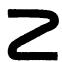
\includegraphics[keepaspectratio]{images/part002_287b28a9.jpg}}

注意这些函数并不是 T 上具紧支集的连续函数。

现在转到积分的定义。

命题 16. --- 存在且只存在一个连续线性映射 \(\mathbf{f} \mapsto \int \mathbf{f} d\mu\) ，它把空间 \(\overline{\mathcal{L}}_{\mathrm{F}}^{1}(\mu)\) 映到 \(\mathrm{F}\) 中，具有下列性质：

若 \(\mathbf{f}\) 形如 \(t \mapsto g(t)\mathbf{a}\) ，其中 \(\mathbf{a} \in \mathbf{F}\) ，\(g\) 是有限、\(\mu\) -可测的正函数且 \(\mu^{\bullet}(g) < +\infty\) ，则 \(\int \mathbf{f} d\mu = \mu^{\bullet}(g) \cdot \mathbf{a}\) 。

因为半范数空间 \(\overline{\mathcal{L}}_{\mathrm{F}}^{1}(\mu)\) 与 \(\overline{\mathcal{L}}_{\mathrm{F}}^{1}(\mu')\) 相同。由于 \(\mu^{\bullet} = \mu'^{\bullet}\) ，映射 \(\mathbf{f} \mapsto \int \mathbf{f} d\mu'\) 满足陈述中的条件。另一方面，陈述中所考虑的形如 \(\mathbf{f} = g \cdot \mathbf{a}\) 的函数全体在 \(\overline{\mathcal{L}}_{\mathrm{F}}^{1}(\mu')\) 中完全 (Ch. IV, §3, No.~5, Prop. 10)，由此得唯一性。

称 \(\int f d\mu\) 为 f 关于 \(\mu\) 的积分，这个向量也记作 \(\mu(\mathbf{f})\) 或 \(\int \mathbf{f}(t) d\mu(t)\) 。

由于对每个以 F 为值的本性可积函数 f 有 \(\int f d\mu = \int f d\mu'\) ，本质积分的全部理论无需新证明即可推广到 Hausdorff 空间上的测度；由它出发，把自身限制于适度函数，便得到关于通常积分的结果。我们特别引用下列结果：

--- Ch. IV, §3, No.~4 的 Th. 3，它到 \(\overline{\mathcal{L}}_{\mathrm{F}}^{p}\) 的推广，以及它的两个推论。

--- Ch. IV, §3, No.~5 的 Th. 4（与连续线性映射的复合）及其推论；同一 No. 的 Props. 9、11 与 12。

--- Ch. IV, §3, No.~6 中关于 \(L^{p}\) 的序向量空间结构的全部结果。

--- Ch. IV, §3, No.~7 的全部结果，特别是 Lebesgue 定理。

--- Ch. IV, §3, No.~8 中关于空间 \(L_F^p\) 之间关系的全部结果。

--- Ch. IV, §4, No.~3 的 Theorem 2（Lebesgue 定理对 \(L_F^1\) 的特殊陈述）。

--- Hölder 不等式 (Ch. IV, §6, No.~4, Th. 2) 及其推论。

--- Ch. IV, §6, No.~5 中建立的空间 \(L_{F}^{p}\) 之间的关系。

-- Ch. V, §5, No.~8 中建立的空间 \(\mathbf{L}^p\) 的对偶性结果。

--- Dunford--Pettis 定理 (Ch. VI, §2, No.~5, Th. 1)、其 Corollaries 1 与 2，以及 Ch. VI, §2, No.~6 的 Prop. 10（\(L_{F}^{1}\) 的对偶）。

\section{测度的运算}

与前节一样，T 表示一个 Hausdorff 拓扑空间，\(\mu\) 表示 T 上的一个测度。回顾：除非另有说明，所有测度都假定为正的。

\subsection{可测子空间上的诱导测度}

设 X 是 T 的子集，\(\nu\) 是映射 \(\mu: K \mapsto \mu_{K}\) 在 X 的紧子集全体上的限制；显然 \(\nu\) 是 X 上的一个前测度。另一方面，设 \(x \in X\) ，V 是 \(x\) 在 \(\mathbf{T}\) 中的开邻域且 \(\mu^{\bullet}(\mathrm{V}) < +\infty\) ；则

\[
\nu^{\bullet}(\mathrm{X}\cap \mathrm{V}) = \sup_{\substack{\mathrm{K\ compact}\\ \mathrm{K}\subset \mathrm{X}\cap \mathrm{V}}}\mu^{\bullet}(\mathrm{K})\leqslant \mu^{\bullet}(\mathrm{V}) <   + \infty
\]

（由 §1, No.~2 的注 3），因此 \(\nu\) 是一个测度。

当 X 不是 \(\mu\) -可测的时，负担 \(\nu^{\bullet}\) 与 \((\mu^{\bullet})_{X}\) 未必相等，测度 \(\nu\) 也并不令人感兴趣。

定义 1. --- 设 X 是 T 的 \(\mu\) -可测子集。\(\mu: \mathrm{K} \mapsto \mu_{\mathrm{K}}\) 在 X 的紧子集全体上的限制称为 \(\mu\) 在子空间 X 上诱导的测度，记作 \(\mu_{\mathrm{X}}\) 或 \(\mu|_{\mathrm{X}}\) 。

命题 1. --- 设 X 是 T 的 \(\mu\) -可测子集。负担 \((\mu_{\mathrm{X}})^{\bullet}\) 等于负担 \((\mu^{\bullet})_{\mathrm{X}}\) ——由 \(\mu^{\bullet}\) 在 X 上诱导——(§1, No.~1)。换言之，有 \((\mu_{\mathrm{X}})^{\bullet}(g) = \mu^{\bullet}(g^{0})\) （对每个函数 \(g \in \mathcal{F}_{+}(\mathrm{X})\)）。

设 \(f \in \mathcal{F}_{+}(X)\) ，\(f^{0}\) 是 \(f\) 到 \(T\) 上经 0 的延拓。有 \((\mu^{\bullet})_{X}(f) = \mu^{\bullet}(f^{0}) = \sup_{L} \mu^{\bullet}(f^{0}\varphi_{L})\) ，其中 \(L\) 取遍 \(T\) 的紧子集全体 (§1, No.~2, Prop. 2)；类似地 \((\mu_{X})^{\bullet}(f) = \sup_{K} \mu_{K}^{\bullet}(f_{K}) = \sup_{K} \mu^{\bullet}(f^{0}\varphi_{K})\) ，其中 \(K\) 取遍 \(X\) 的紧子集全体。于是问题归结为证明 \(\mu^{\bullet}(f^{0}\varphi_{L}) = \sup_{K} \mu^{\bullet}(f^{0}\varphi_{K})\) 对每个紧子集 \(L\) ⊂ \(T\) 成立，其中 \(K\) 取遍 \(L \cap X\) 的紧子集全体。现设 \((K_{n})\) 是含于 \(L \cap X\) 的递增紧集序列，使 \((L \cap X) - \bigcup_{n} K_{n}\) 局部 \(\mu\) -可忽略 (§1, No.~8, Prop. 11)；由于 \(f^{0}\) 在 \(X\) 外为零，\(f^{0}\varphi_{L}\) 在 \(L \cap X\) 外为零，故局部几乎处处等于序列 \((f^{0}\varphi_{K_{n}})\) 的上包络。由此推出 \(\mu^{\bullet}(f^{0}\varphi_{L}) = \sup \mu^{\bullet}(f^{0}\varphi_{K_{n}})\) ，从而得到所要的结果。

注 3). --- 设 X 是 T 的 \(\mu\) -可测子集。把 §1, No.~8 的 Prop. 10 应用于 \(g = \varphi_{\mathbf{X}}\) ，存在 T 的一个破碎 \((\mathrm{K}_{\alpha})_{\alpha \in \mathbf{A}}\) ，使对每个 \(\alpha \in \mathbf{A}\) ，或者 \(\mathrm{K}_{\alpha} \subset \mathrm{X}\) ，或者 \(\mathrm{K}_{\alpha} \subset \mathbb{C}\mathrm{X}\) 。若按 §1, No.~8 的附论的程序修改 T 的拓扑，则空间 \(\mathrm{X}'\) ——由给 X 赋予 \(\mathrm{T}'\) 诱导的拓扑而得到——是局部紧的，并且我们知道如何对 \(\mu\) （相应地对 \(\mu_{\mathbf{X}}\) ）联系一个测度 \(\mu'\) （相应地 \(\nu\) ），它在 \(\mathrm{T}'\) 上（相应地在 \(\mathrm{X}'\) 上），它与 \(\mu\) （相应地 \(\mu_{\mathbf{X}}\) ）有相同的本质上积分：这蕴含 \(\mu'_{\mathbf{X}'} = \nu\) 。由于局部可忽略集、可测映射以及以 Banach 空间为值的本性可积函数对 \(\mu\) 与 \(\mu'\) 相同，且对 \(\mu_{\mathbf{X}}\) 与 \((\mu_{\mathbf{X}})' = \nu = \mu'_{\mathbf{X}'}\) 相同，关于诱导测度的积分理论就化归为 Ch. V, §7 在局部紧空间这一特殊情形中处理过的理论。结果的改写留给读者。
